\documentclass[russian,utf8,12pt]{eskdtext}
\usepackage[numbertop, numbercenter]{eskdplain}

% - Подключаем шрифты из пакета scalable-cyrfonts-tex
\usepackage{cyrtimes}

% - Отступ красной строки
\setlength{\parindent}{1.25cm}

% - Убирает точку в списке литературы
\makeatletter
\def\@biblabel#1{#1 }

% - Точки для всех пунктов в оглавлении
\renewcommand*{\l@section}{\@dottedtocline{1}{1.5em}{2.3em}}
\renewcommand*{\l@subsection}{\@dottedtocline{1}{1.5em}{2.3em}}
\renewcommand*{\l@subsubsection}{\@dottedtocline{1}{1.5em}{2.3em}}

% - Для переопределения списков
\renewcommand{\theenumi}{\arabic{enumi}}
\renewcommand{\labelenumi}{\theenumi)}
\makeatother

\usepackage{enumitem}
\setlist{nolistsep, itemsep=0.3cm,parsep=0pt}

% - ГОСТ списка литературы
\bibliographystyle{utf8gost705u}

% - Верикальные отступы заголовков 
\ESKDsectSkip{section}{1em}{1em}
\ESKDsectSkip{subsection}{1em}{1em}
\ESKDsectSkip{subsubsection}{1em}{1em}

% - Изменение заголовков
\usepackage{titlesec}
\titleformat{\section}{\centering\normalfont\normalsize}{\thesection}{1.0em}{}
\titleformat{\subsection}{\centering\normalfont\normalsize}{\thesubsection}{1.0em}{}
\titleformat{\subsubsection}{\centering\normalfont\normalsize}{\thesubsubsection}{1.0em}{}
\titleformat{\paragraph}{\centering\normalsize}{\theparagraph}{1.0em}{}

% - Оставим место под ТЗ 
%\setcounter{page}{4}

% - Для больших таблиц
\usepackage{longtable}
\usepackage{tabularx}
\renewcommand{\thetable}{\thesection.\arabic{table}}

% - Используем графику в документе
\usepackage{graphicx}
\graphicspath{{images/}}
\renewcommand{\thefigure}{\thesection.\arabic{figure}}

% - Счётчики
\usepackage{eskdtotal}

% - Выравнивание по ширине
\sloppy

% - Разрешить перенос двух последних букв слова
\righthyphenmin=2

\RequirePackage{enumitem}
\renewcommand{\alph}[1]{\asbuk{#1}}
\setlist{nolistsep}
\setitemize[1]{label=--, fullwidth, itemindent=\parindent, 
  listparindent=\parindent}% для дефисного списка
\setenumerate[1]{label=\arabic*), fullwidth, itemindent=\parindent, 
  listparindent=\parindent}% для нумерованного списка
\setenumerate[2]{label=\alph*), fullwidth, itemindent=\parindent, 
  listparindent=\parindent, leftmargin=\parindent}% для списка 2-ой ступени, который будет нумероваться а), б) и т.д.

\usepackage{listings}  
\lstset{basicstyle=\ttfamily\small}

\begin{document}
 \newpage
\ESKDthisStyle{empty}

\begin{center}
 Министерство образования и науки Российской Федерации\\
 Федеральное государственное бюджетное образовательное учреждение высшего профессионального образования\\
 <<ТОМСКИЙ ГОСУДАРСТВЕННЫЙ УНИВЕРСИТЕТ СИСТЕМ УПРАВЛЕНИЯ И РАДИОЭЛЕКТРОНИКИ>> (ТУСУР)\\
 Кафедра комплексной информационной безопасности электронно-вычислительных систем (КИБЭВС)\\
\end{center}

\vfill

\begin{flushright}
\begin{minipage}{0.45\textwidth}
 \begin{flushleft}
  УТВЕРЖДАЮ\\
  заведующий каф. КИБЭВС
  \underline{\hspace{3cm}}А.А. Шелупанов \\
  <<\underline{\hspace{1cm}}>>\underline{\hspace{3cm}}2016г.\\
 \end{flushleft}
\end{minipage}
\end{flushright}

\vfill

\begin{center}
КОМПЬЮТЕРНАЯ ЭКСПЕРТИЗА

Отчет по групповому проектному обучению

Группа КИБЭВС-1401
\end{center}

\vfill
\begin{flushright}
\begin{minipage}{0.45\textwidth}
 \begin{flushleft}
  Ответственный исполнитель \\
  студент гр. 722 \\
  \underline{\hspace{3cm}}О.В. Лобанов \\
  <<\underline{\hspace{1cm}}>>\underline{\hspace{3cm}}2016г.\\
 \end{flushleft}
\end{minipage}
\end{flushright}

\vfill

\begin{flushright}
\begin{minipage}{0.45\textwidth}
 \begin{flushleft}
  Научный руководитель \\
  аспирант каф. КИБЭВС \\
  \underline{\hspace{3cm}}А.И. Гуляев \\
  <<\underline{\hspace{1cm}}>>\underline{\hspace{3cm}}2016г.\\
 \end{flushleft}
\end{minipage}
\end{flushright}

\vfill

\begin{center}
 2016
\end{center}

 \newpage
\ESKDthisStyle{empty}
\paragraph{\hfill РЕФЕРАТ \textbf{ПРАВИТЬ!!!} \hfill}
Курсовая работа содержит \ESKDtotal{page} страниц, \ESKDtotal{figure} рисунка, \ESKDtotal{table} таблицы, \ESKDtotal{bibitem} источников, \ESKDtotal{appendix} приложение.

%допилить ключевые слова
КОМПЬЮТЕРНАЯ ЭКСПЕРТИЗА, ФОРЕНЗИКА, ЛОГИ, QT, XML, GIT, LATEX, ICQ, MS OUTLOOK, WINDOWS, PST, MSG, RTF, HTML, БИБЛИОТЕКИ, РЕПОЗИТОРИЙ, МЕССЕНДЖЕР, ПОЧТОВЫЙ КЛИЕНТ, SQLLITE, РЕЕСТР, ИЗОБРАЖЕНИЯ, READPST, JPEG, PNG.

Цель работы --- создание программного комплекса, предназначенного для проведения компьютерной экспертизы.

Задачей, поставленной на данный семестр, стало написание программного комплекса, имеющего следующие возможности: 
\begin{enumerate}
\item сбор и анализ информации из реестра;
\item сбор и анализ информации из журналов истории браузеров;
\item сбор и анализ информации из мессенджеров;
\item сбор и анализ информации из почтовых приложений;
\item идентификации файлов изображений по внутреннему содержимому и их проверка;
\item сбора информации об установленном ПО по остаточным файлам.
\end{enumerate}

Результаты работы в данном семестре:

\begin{itemize}
\item реализован алгоритм извлечения строковых переменных из реестра Windows;
\item реализован алгоритм побитового считывания файла формата PST;
\item реализован импорт истории (посещений, поисковых запросов, загруженных файлов), закладок и 
другой информации (версия приложения, логин аккаунта google) из приложения Google Chrome;
\item реализован алгоритм парсинга контактного листа пользователя, сохраняемого приложением ICQ;
\item реализована проверка конца файла для форматов JPEG и PNG (для идентификации файлов изображений) и проверка заголовков 5 форматов изображений;
\end{itemize}

Пояснительная записка выполнена при помощи системы компьютерной вёрстки \LaTeX.

 
 \newpage
 \ESKDthisStyle{empty}
 \section*{Список исполнителей}
 
Лобанов О.В. -- программист, ответственный исполнитель, ответственный за разработку функций сбора информации из реестра. 

Шиповской В.В. -- программист, ответственный за написание части системы для сбора и обработки информации из браузера Google Chrome.

Серяков А.В. -- программист, ответственный за написание части системы для сбора информации из почтового клиента MS Outlook.

Боков И.М. -- программист, ответственный за написание части системы для для нахождения медиа-файлов (аудио, видео, изображение) и извлечения мета-данных из них.

Кучер М.В. -- программист, ответственный за написание части системы для сбора информации об установленном ПО по остаточным файлам.

Терещенко Ю.А. -- программист, ответственный за написание части системы для сбора информации из почтового клиента Mozilla Thunderbird.

Мейта М.В. -- документатор, ответсвенный за верстку необходимой документации в системе \TeX.

 
 % - содержание
 \newpage
 \ESKDstyle{plain}
 \tableofcontents

 \newpage
 \ESKDstyle{plain}
 \section*{Введение}
 \addcontentsline{toc}{section}{Введение}
 Компьютерно-техническая экспертиза является классом инженерно-\\технических экспертиз, проводимых в целях поиска криминалистически значимой информации на носителях, её всестороннего исследование, и, как следствие, получения доказательственной информации и установления фактов, имеющих значение для уголовных, гражданских и административных дел, сопряжённых с использованием компьютерных технологий. Для проведения компьютерных экспертиз необходима высокая квалификация экспертов, так как при изучении представленных носителей информации, попытке к ним доступа и сбора информации возможно внесение в информационную среду изменений или полная утрата важных данных.

Компьютерная экспертиза, в отличие от компьютерно-технической экспертизы, затрагивает только информационную составляющую, в то время как аппаратная часть и её связь с программной средой не рассматривается.

На протяжении предыдущих семестров нами были рассмотрены такие направления компьютерной экспертизы, как исследование файловых систем, сетевых протоколов, организация работы серверных систем, механизм журналирования событий. Также нами были изучены основные задачи, которые ставятся перед сотрудниками правоохранительных органов, которые проводят компьютерную экспертизу, и набор чуществующих утилит, способных помочь эксперту в проведении компьютерной экспертизы. Было выявлено, что существует множество разрозненных программ, предназначенных для просмотра лог-файлов системы и таких приложений, как мессенджеры и браузеры, но для каждого вида лог-файлов необходимо искать отдельную программу. Так как ни одна из них не позволяет эксперту собрать воедино и просмотреть все логи системы, браузеров и мессенджеров, было решено создать для этой цели собственный автоматизированный комплекс, которому на данный момент нет аналогов.


 \section{Назначение и область применения}
Разрабатываемый комплекс предназначен для автоматизации процесса сбора информации с исследуемого образа жёсткого диска.
\section{Постановка задачи}
\setcounter{figure}{0}
На данный семестр были поставлены следующие задачи:

\begin{itemize}
\item изучение архитектуры проекта <<Компьютерная экспертиза>> новыми участниками проектной группы;
\item изучение теоретического материала и основных инструментов разработки;
\item определение индивидуальных задач для каждого участника проектной группы;
\item исследование предметных областей в рамках индивидуальных задач; 
\item реализация новых программных модулей и доработка уже существующих;
\item изучение инструментов для генерации документации к программному коду проекта.
\end{itemize}

Задачи по проектированию модулей:

\begin{enumerate}
\item сбор и анализ информации из реестра Windows;
\item сбор и анализ информации из браузера Google Chrome;
\item сбор и анализ информации из почтового клиента Mozilla Thunderbird;
\item сбор и анализ информации из почтового клиента MS Outlook;
\item поиск медиа-файлов (аудио, видео, изображение) и извлечение мета-данных из них;
\item сбор информации об установленном ПО по остаточным файлам.
\end{enumerate}

\section{Инструменты}
\setcounter{figure}{0}
\subsection{Система контроля версий Git}
Для разработки программного комплекса для проведения компьютерной экспертизы было решено использовать Git.

Git --- распределённая система управления версиями файлов. Проект был создан Линусом Торвальдсом для управления разработкой ядра Linux  как противоположность  системе управления версиями Subversion (также известная как «SVN»). \cite{progit}

При работе над одним проектом команде разработчикоа необходим инструмент для совместного написания, бэкапирования и тестирования программного обеспечения. Используя Git, мы имеем:
\begin{itemize}
\item возможность удаленной работы с исходными кодами;
\item возможность создавать свои ветки, не мешая при этом другим разработчикам;
\item доступ к последним изменениям в коде, т.к. все исходники хранятся на сервере git.keva.su;
\item исходные коды защищены, доступ к ним можно получить лишь имея RSA-ключ;
\item возможность откатиться к любой стабильной стадии проекта.
\end{itemize}

Основные постулаты работы с кодом в системе Git:

\begin{itemize}
\item каждая задача решается в своей ветке;
\item необходимо делать коммит как только был получен осмысленный результат;
\item ветка master мержится не разработчиком, а вторым человеком, который производит вычитку и тестирование изменения;
\item все коммиты должны быть осмысленно подписаны/прокомментированы.
\end{itemize}


\subsection{Система компьютерной вёрстки \TeX}
\TeX\ --- это созданная американским математиком и программистом Дональдом Кнутом система для вёрстки текстов. Сам по себе \TeX\ представляет собой специализированный язык программирования.Каждая издательская система представляет собой пакет макроопределений этого языка.

\LaTeX\ --- это созданная Лэсли Лэмпортом издательская система на базе \TeX'а \cite{lvovskyi} \LaTeX\ позволяет пользователю сконцентрировать свои услия на содержании и структуре текста, не заботясь о деталях его оформления.

Для подготовки отчётной и иной документации нами был выбран \LaTeX\, так как совместно с системой контроля версий Git он предоставляет возможность совместного создания и редактирования документов. Огромным достоинством системы \LaTeX\ то, что создаваемые с её помощью файлы обладают высокой степенью переносимости. \cite{latexrus}

Совместно с \LaTeX\ часто используется Bib\TeX\ --- программное обеспечение для создания форматированных списков библиографии. Оно входит в состав дистрибутива \LaTeX\ и позволяет создавать удобную, универсальную и долговечную библиографию. Bib\TeX\ стал одной из причин, по которой нами был выбран \LaTeX\ для создания документации.

\subsection{Система документирования Doxygen}
Doxygen --- это кроссплатформенная система документирования исходных текстов, которая поддерживает разлличные языки программирования (в том числе и C++) \cite{doxygen}. 

Doxygen генерирует документацию на основе набора исходных текстов и также может быть настроен для извлечения структуры программы из недокументированных исходных кодов. Возможно составление графов зависимостей программных объектов, диаграмм классов и исходных кодов с гиперссылками.

Doxygen имеет встроенную поддержку генерации документации в формате HTML, \LaTeX\, man, RTF и XML. Также вывод может быть легко сконвертирован в CHM, PostScript, PDF.

Doxygen — консольная программа в духе классической Unix. Она работает подобно компилятору, анализируя исходные тексты и создавая документацию. Параметры создания документации читаются из конфигурационного файла, имеющего простой текстовый формат.

Автором программы является голландец Димитри ван Хееш (Dimitri van Heesch).

\subsection{Qt - кроссплатформенный инструментарий разработки ПО}
Qt --- это кроссплатформенная библиотека C++ классов для создания графических пользовательских интерфейсов (GUI) от фирмы Digia. Эта библиотека полностью объектно-ориентированная, что обеспечивает легкое расширение возможностей и создание новых компонентов. Ко всему прочему, она поддерживает огромнейшее количество платформ.

Qt позволяет запускать написанное с его помощью ПО в большинстве современных операционных систем путём простой компиляции программы для каждой ОС без изменения исходного кода. Включает в себя все основные классы, которые могут потребоваться при разработке прикладного программного обеспечения, начиная от элементов графического интерфейса и заканчивая классами для работы с сетью, базами данных и XML. Qt является полностью объектно-ориентированным, легко расширяемым и поддерживающим технику компонентного программирования.

Список использованных классов фраемворка QT
\begin{itemize}
\item iostream
\item QChar
\item QCryptographicHash
\item QDateTime
\item QDir
\item QDirIterator
\item QFile
\item QFileInfo
\item QIODevice
\item QList
\item QRegExp
\item QString
\item QTextStream
\item QtSql/QSqlDatabase
\item QVector
\item QMap
\item QXmlStreamReader
\item QXmlStreamWriter
\item Conversations
\end{itemize}

Класс QXmlStreamWriter представляет собой XML писателя с простым потоковым.

Класс QXmlStreamReader представляет собой быстрый синтаксически корректный XML анализатор с простым потоковым API. 

QVector представляет собой класс для создания динамических массивов.

Модуль QtSql/QSqlDatabase помогает обеспечить однородную интеграцию БД в ваши Qt приложения.

Класс QTextStream предоставляет удобный интерфейс для чтения и записи текста.

QTextStream может взаимодействовать с QIODevice, QByteArray или QString. Используя потоковые операторы QTextStream, вы можете легко читать и записывать слова, строки и числа. При формировании текста QTextStream поддерживает параметры форматирования для заполнения и выравнивания полей и форматирования чисел. \cite{qtdoc}

Класс QString предоставляет строку символов Unicode.

Класс QMap --- контейнерный класс для хранения элементов различных типов данных.

Класс QDateTime используется для работы с форматом даты, в который записывается информация о файле.

QString хранит строку 16-битных QChar, где каждому QChar соответствует один символ Unicode 4.0. (Символы Unicode со значениями кодов больше 65535 хранятся с использованием суррогатных пар, т.е. двух последовательных QChar.)

Unicode - это международный стандарт, который поддерживает большинство использующихся сегодня систем письменности. Это расширение US-ASCII (ANSI X3.4-1986) и Latin-1 (ISO 8859-1), где все символы US-ASCII/Latin-1 доступны на позициях с тем же кодом.

Внутри QString использует неявное совместное использование данных (копирование-при-записи), чтобы уменьшить использование памяти и избежать ненужного копирования данных. Это также позволяет снизить накладные расходы, свойственные хранению 16-битных символов вместо 8-битных.

В дополнение к QString Qt также предоставляет класс QByteArray для хранения сырых байт и традиционных нультерминальных строк. В большинстве случаев QString - необходимый для использования класс. Он используется во всем API Qt, а поддержка Unicode гарантирует, что ваши приложения можно будет легко перевести на другой язык, если в какой-то момент вы захотите увеличить их рынок распространения. Два основных случая, когда уместно использование QByteArray: когда вам необходимо хранить сырые двоичные данные и когда критично использование памяти (например, в Qt для встраиваемых Linux-систем). \cite{qtcross}

Класс QRegExp предоставляет сопоставление с образцом при помощи регулярных выражений.

Регулярное выражение, или ''regexp'', представляет собой образец для поиска соответствующей подстроки в тексте. Это полезно во многих ситуациях, например:

Проверка правильности -- регулярное выражение может проверить, соответствует ли подстрока каким-либо критериям, например, целое ли она число или не содержит ли пробелов.
Поиск -- регулярное выражение предоставляет более мощные шаблоны, чем простое соответствие строки, например, соответствие одному из слов mail, letter или correspondence, но не словам email, mailman, mailer, letterbox и т.д.
Поиск и замена -- регулярное выражение может заменить все вхождения подстроки другой подстрокой, например, заменить все вхождения \& на \&amp;, исключая случаи, когда за \& уже следует amp;.
Разделение строки -- регулярное выражение может быть использовано для определения того, где строка должна быть разделена на части, например, разделяя строку по символам табуляции.

QFileInfo  - Во время поиска возвращает полную информацию о файле.

Класс QDir обеспечивает доступ к структуре каталогов и их содержимого.

QIODevice представляет собой базовый класс всех устройств ввода/вывода в Qt.

Класс QCryptographicHash предоставляет способ генерации криптографических хэшей.
QCryptographicHash могут быть использованы для генерации криптографических хэшей двоичных или текстовых данных.В настоящее время MD4, MD5, и SHA-1 поддерживаются. \cite{qtcross}

QChar обеспечивает поддержку 16-битных символов Unicode.

\subsubsection{Aвтоматизация поиска журнальных файлов}

Для сканирования образа на наличие интересующих лог файлов использовался класс QDirIterator. После вызова происходит поочередный обход по каждому файлу в директории и поддиректории. Проверка полученного полного пути к файлу осуществляется регулярным выражением, если условие выполняется, происходит добавление в список обрабатываемых файлов.

\subsubsection{Реализация сохранения результатов работы программного комплекса в XML}

Cохранение полученных данных происходит в ранее выбранный формат XML(Extensible Markup Language). Для этого используется класс QXmlStreamReader и QxmlStreamWriter.
Класс QXmlStreamWriter представляет XML писателя с простым потоковым API.

QXmlStreamWriter работает в связке с QXmlStreamReader для записи XML. Как и связанный класс, он работает с QIODevice, определённым с помощью setDevice().

Сохранение данных реализованно в классе WriteMessage. В методе WriteMessages, структура которого представлена на UML диаграмме в разделе Архитектура.


\section{Технические характеристики}
\section {Технические характеристики}

%я не уверен, но помоему этот раздел надо бы подругому назвать =) 

\subsection {Постановка задачи}

На данный семестр были поставлены следующие задаи:

\begin{enumerate}
\item Определиться при помощи каких средств вести разработку
\item Разработать архитектуру проекта
\item Реализовать структуру проекта 
\item Определиться с форматом выходных данных
\item Реализовать несколько модулей
\end{enumerate}

\subsection {Выбор единого формата выходных файлов}

Для вывода результата был выбран формат XML-документов, так как с данным форматом лего работать при помощи программ, а результат работы данного комплекса в дальнейшем планируется обрабатывать при помощи программ

%и вот тут вброс про XML можно.

\subsubsubsubsection {Требования к аппаратному обеспечению}

Минимальные системные требования:\\
- Процессор 1ГГц Pentium 4;\\
- память 512 Мб;\\
- диск 9 Гб.

\subsubsubsubsection {Требования к программному обеспечению обеспечению}

На компьютерне должна быть установлена операционная система ubuntu 12.04 или выше, данная система должна иметь набор библиотек QT.
\subsection{Выбор единого формата выходных файлов}
Для вывода результата был выбран формат XML-документов, так как с данным форматом лего работать при помощи программ, а результат работы данного комплекса в дальнейшем планируется обрабатывать при помощи программ.

XML - eXtensible Markup Language или расширяемый язык разметки. Язык XML представляет собой простой и гибкий текстовый формат, подходящий в качестве основы для создания новых языков разметки, которые могут использоваться в публикации документов и обмене данными \cite{xml}. Задумка языка в том, что он позволяет дополнять данные метаданными, которые разделяют документ на объекты с атрибутами. Это позволяет упростить программную обработку документов, так как структурирует информацию.

Простейший XML-документ может выглядеть так:


\begin{verbatim}
<?xml version="1.0"?>
<list_of_items>
<item id="1"\><first/>Первый</item\>
<item id="2"\>Второй <subsub_item\>подпункт 1</subsub_item\></item\>
<item id="3"\>Третий</item\>
<item id="4"\><last/\>Последний</item\>
</list_of_items>
\end{verbatim}


Первая строка - это объявление начала XML-документа, дальше идут элементы документа <list\_of\_items> - тег описывающий начало элемента \\list\_of\_items, </list\_of\_items> - тег конца элемента. Между этими тегами заключается описание элемента, которое может содержать текстовую информацию или другие элементы (как в нашем примере). Внутри тега начала элемента так же могут указывать атрибуты элемента, как например атрибут id элемента item, атрибуту должно быть присвоено определенное значение.


\section{Разработка программного обеспечения}
\setcounter{figure}{0}
 
\subsection{Архитектура}
\subsection{Основной алгоритм}
В ходе разарботки был применен видоизменнённый шаблон проектирования Factory method.

%Описание шаблона и его модификации
Данный шаблон относится к классу порождающих шаблонов. Шаблоны данного класса - это шаблоны проектирования, которые абстрагируют процесс инстанцирования (создания экземпляра класса). Они позволяют сделать систему независимой от способа создания, композиции и представления объектов. Шаблон, порождающий классы, использует наследование, чтобы изменять инстанцируемый класс, а шаблон, порождающий объекты, делегирует инстанцирование другому объекту.
Основной алгоритм представлен на рисунке \ref{architech:architech}.

\begin{figure}[h!]
\center{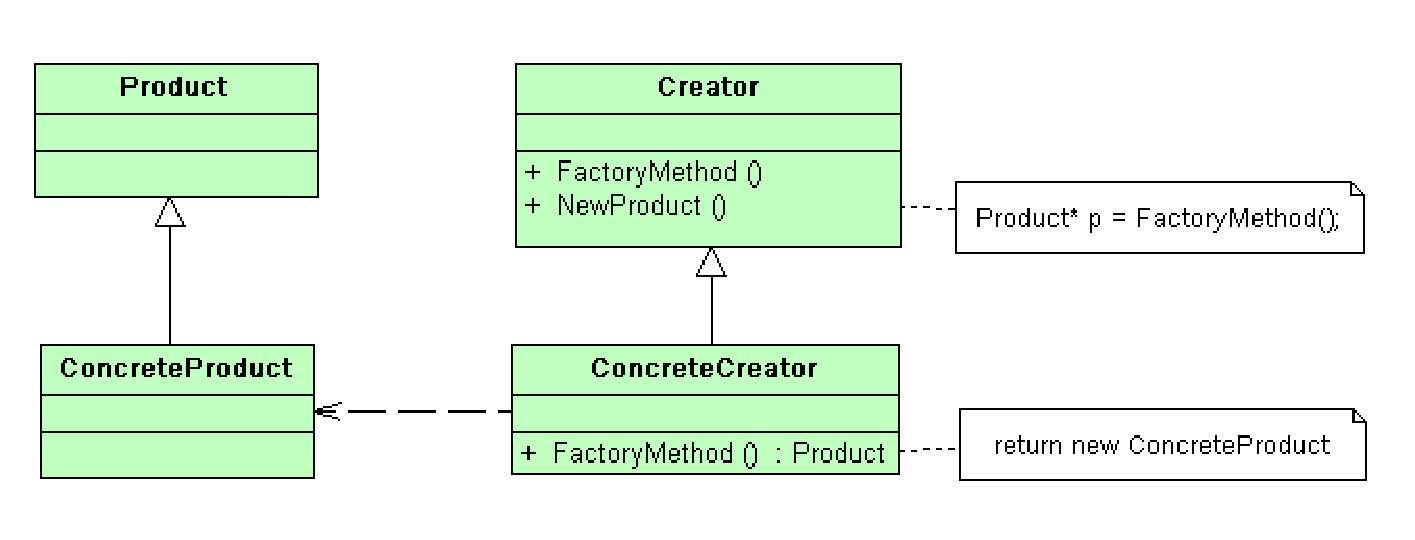
\includegraphics[width=0.9\linewidth]{architech}}
\caption{Основной алгоритм}
\label{architech:architech}
\end{figure}

Использование данного шаблона позволило нам разбить наш проект на независимые модули, что весьма упростило задачу разработки, так как написание алгоритма для конкретного таска не влияло на остальную часть проекта. При разработке был реализован базовый класс для работы с образом диска. Данный клас предназначался для формирования списка настроек, определения операционной системы на смонтированном образе и инстанционировании и накапливание всех необходимых классов-тасков в очереди тасков. После чего каждый таск из очереди отправлялся на выполнение. Блоксхема работы алгоритма (тут картинка alg_main.eps)

Каждый класс-таск порождался путем наследования от базового абстрактного класса который имеет 8 методов и 3 атрибута:

\begin{enumerate}
\item QString manual() - возвращает справку о входных параметрах данного таска;
\item void setOption(QStringList list) - установка флагов для поданных на вход параметров;
\item QString command() - возвращает команду для инициализации такска вручную;
\item bool supportOS(const coex::typeOS \&os) - возвращает флаг, указывающий на возможность использования данного таска для конкретной операционной системы;
\item QString name() - возвращает имя данного таска;
\item QString description() - возвращает краткое описание таска;
\item bool test() - предназначена для теста на доступность таска;
\item bool execute(const coex::config \&config) - запуск таска на выполнение;
\item QString m\_strName - хранит имя таска;
\item QString m\_strDescription - хранит описание таска;
\item bool m\_bDebug - флаг для параметра --debug;
\end{enumerate}

На данный момент в проекте используется восемь классов. UML-диаграмма классов представлена на рисунке (тут картинка UML.eps)

Классы taskSearchSyslogsWin, taskSearchPidginWin и taskSearchSkypeWin - наследники от класса task являются тасками. Класс winEventLog и _EVENTLOGRECORD предназначины для конвертации журнальных файлов операционной системы Windows XP, а класс writerMessages для преобразования истории переписки.

\newpage
\subsection{Сбор информации из браузера Google Chrome} % - Отчёт Влада
Целью работы в текущем семестре являлось исследование журнальных файлов и доработка программного модуля для сбора пользовательских данных приложения Google Chrome и представления их в формате XML.

В ходе изучения работы данного браузера было установлено, что приложение Google Chrome хранит пользовательские данные локально. Адреса директорий, используемых по умолчанию для этих целей Google Chrome можно увидеть в таблице~\ref{tab:tab_1}, пользовательские данные --- в таблице~\ref{tab:tab_2}.

\begin{table}[ht]
\caption{Директории хранения журнальных файлов Chrome}
\label{tab:tab_1}
\begin{center}
\begin{tabularx}{\linewidth}{|l|X|}
\hline
Операционная система & Директория \\
\hline
Linux (Debian) & /home/имя пользователя/.config/google-chrome/Default/ \\
\hline
Win7 & C:\textbackslash Users\textbackslash имя пользователя \textbackslash AppData\textbackslash Local\textbackslash Google \\
 & \textbackslash Chrome\textbackslash User Data\textbackslash Default\textbackslash \\
\hline
Win8 & C:\textbackslash Users\textbackslash имя пользователя \textbackslash AppData\textbackslash Local\textbackslash Google \\
 & \textbackslash Chrome\textbackslash User Data\textbackslash Default\textbackslash \\
\hline
\end{tabularx}
\end{center}
\end{table}

\begin{table}[ht]
\caption{Пользовательские данные}
\label{tab:tab_2}
\begin{center}
\begin{tabularx}{\linewidth}{|l|X|}
\hline
Файл & Содержание \\
\hline
Bookmarks & Закладки \\
\hline
History & История посещений, история запросов, история загруженных файлов \\
\hline
Preferences & Настройки (директория загрузки файлов, версия программы, логин аккаунта Google) \\
\hline
Login Data & Сохраненные логины и пароли \\
\hline
Extensions (папка) & Расширения \\
\hline
\end{tabularx}
\end{center}
\end{table}

\subsubsection{База данных Login Data Chrome}

Login Data --- это реляционная база данных, основанная на СУБД SQLite.
Необходимо рассмотреть данную БД, которая содержит 2 таблицы:

\begin{enumerate}
  \item logins;
  \item meta.
\end{enumerate}

Интерес представляет только таблица logins. Она содержит следующие поля:

\begin{enumerate}
  \item origin\_url --- адрес ресурса;
  \item username\_value --- логин для доступа;
  \item password\_value --- пароль, представленный в виде BLOB массива двоичных данных (Binary Large OBject);
  \item date\_created --- дата сохранения, представленная в следующем виде (пример): 13072972925957814. Это число есть количество секунд, прошедшее с 00:00:00 UTC 1 января, 1601 года (рис.~\ref{ship_1:ship_1}).
\end{enumerate}

\begin{figure}[h!]
\center{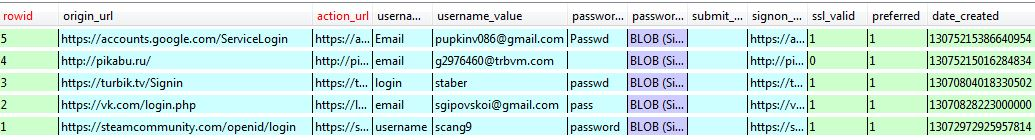
\includegraphics[width=0.9\linewidth]{ship_1}}
\caption{Структура таблицы login}
\label{ship_1:ship_1}
\end{figure} 

Запрос для импорта данных выглядит следующим образом:

\begin{verbatim}
SELECT logins.origin_url,
       logins.username_value,
       datetime(logins.date_created/1000000 + 
       (strftime('%s','1601-01-01')),'unixepoch')
FROM logins;
\end{verbatim}

Результат выполнения запроса можно увидеть на рисунке~\ref{ship_2:ship_2}, блок-схему алгоритма выборки данных из БД Login Data --- на рисунке~\ref{ship_3:ship_3}. Результат выполнения программы в формате XML --- рисунок~\ref{ship_4:ship_4}.

Значение поля id --- уникальный идентификатор для последующего импорта в solr БД и работы с ним.

\begin{figure}[h!]
\center{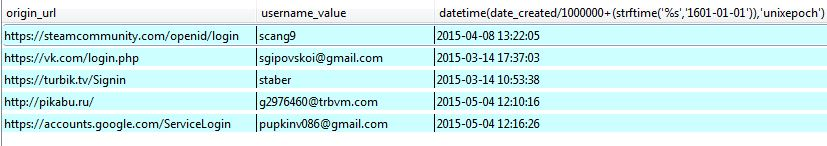
\includegraphics[width=0.9\linewidth]{ship_2}}
\caption{Результат выполнения запроса}
\label{ship_2:ship_2}
\end{figure}

\begin{figure}[h!]
\center{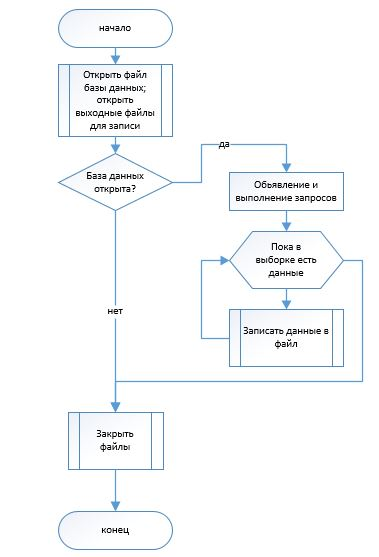
\includegraphics[width=0.5\linewidth]{ship_3}}
\caption{Блок-схема алгоритма выборки данных из БД Login Data}
\label{ship_3:ship_3}
\end{figure} 

\begin{figure}[h!]
\center{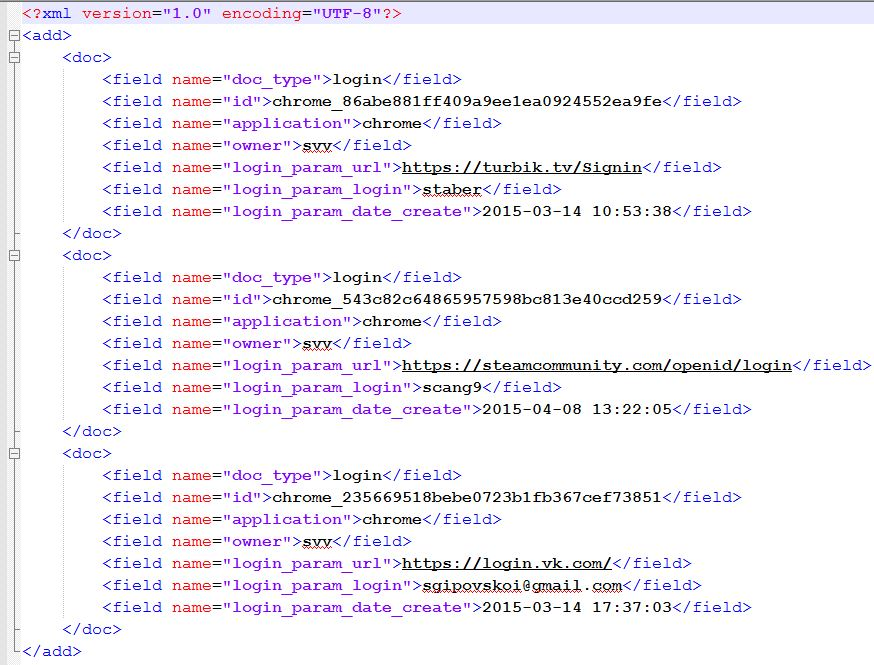
\includegraphics[width=0.7\linewidth]{ship_4}}
\caption{Файл login.XML}
\label{ship_4:ship_4}
\end{figure} 

\clearpage
\subsubsection{Расширения браузера Chrome (Extensions)}

В папке Extensions (рис.~\ref{ship_5:ship_5}) находятся данные об установленных в брузере расширениях. Для каждого расширения имеется своя папка, в которой находится различная информация. Также для каждого Extension имеется файл manifest (рис.~\ref{ship_6:ship_6}) с расширением JSON. JSON (JavaScript Object Notation) --- текстовый формат обмена данными, основанный на JavaScript. Из данного файла необходима только информация об имени и версии расширения.

Блок-схему алгоритма импорта данных о расширениях можно увидеть на рисунке~\ref{ship_7:ship_7}. 

\begin{figure}[h!]
\center{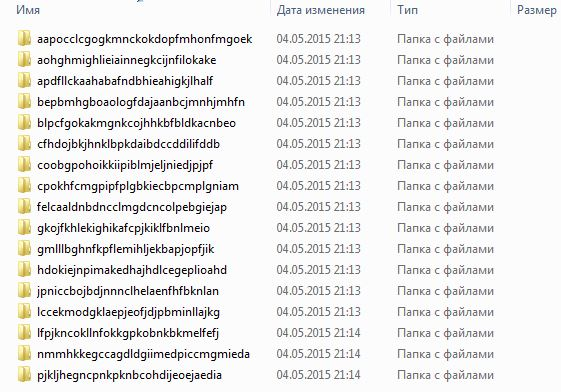
\includegraphics[width=0.6\linewidth]{ship_5}}
\caption{Папка Extensions}
\label{ship_5:ship_5}
\end{figure}

\begin{figure}[h!]
\center{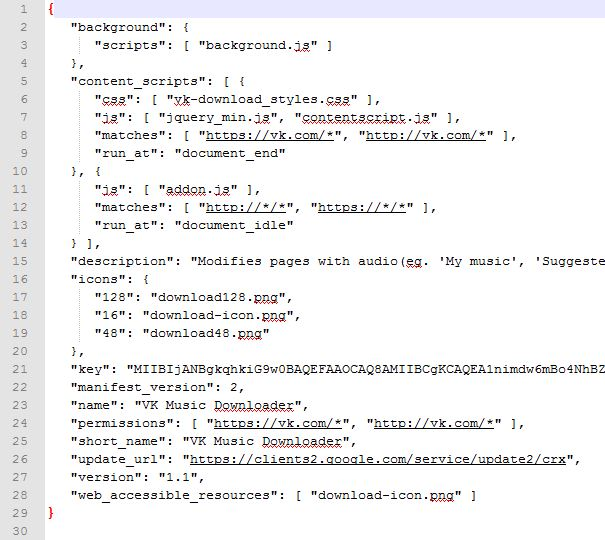
\includegraphics[width=0.6\linewidth]{ship_6}}
\caption{Файл manifest.json}
\label{ship_6:ship_6}
\end{figure}

\begin{figure}[h!]
\center{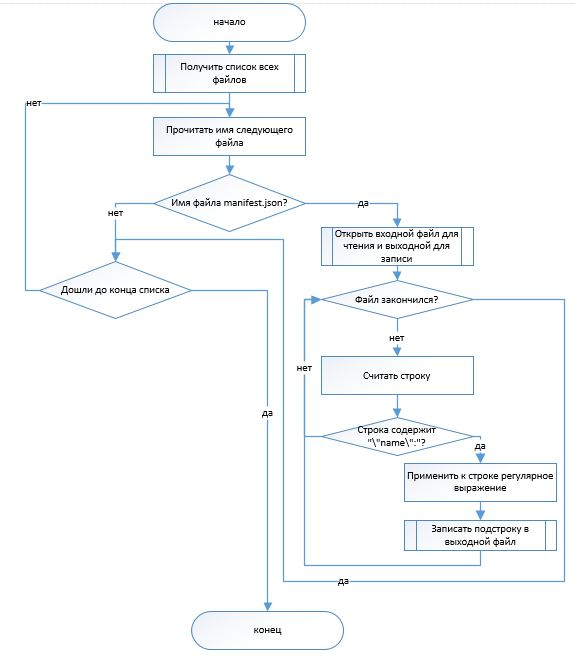
\includegraphics[width=0.8\linewidth]{ship_7}}
\caption{Блок-схема алгоритма импорта данных о расширениях}
\label{ship_7:ship_7}
\end{figure}

\clearpage
Извлечение подстроки из строки осуществляется с помощью регулярного выражения \textbackslash"(.*)\textbackslash".*\textbackslash"(.*)\textbackslash". Например, есть строка <<name>>: <<VK Music Downloader>>. Данное регулярное выражение возвращает 2 подстроки --- <<name>> и <<VK Music Downloader>>, что и требовалось в ходе работы.

Результат был записан в файл extensions.XML (рис.~\ref{ship_8:ship_8}).

\begin{figure}[h!]
\center{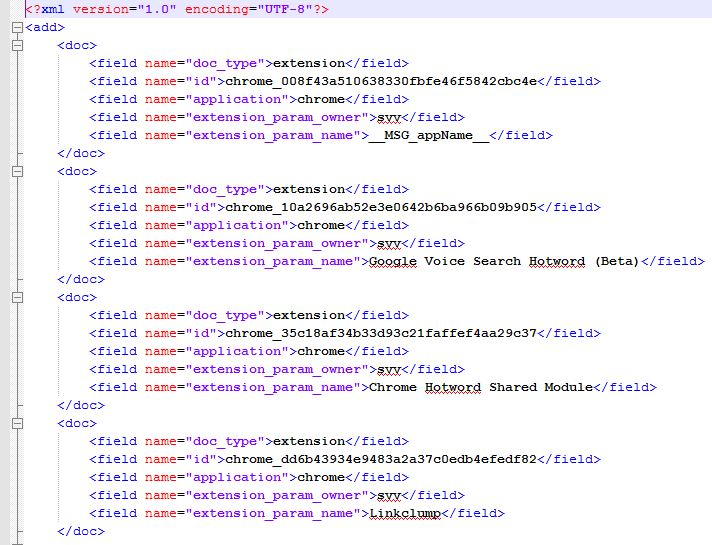
\includegraphics[width=0.7\linewidth]{ship_8}}
\caption{Файл extensions.XML}
\label{ship_8:ship_8}
\end{figure}

\subsubsection{Изменения, добавленные в программный модуль в течение текущего семестра}

В файл bookmarks.XML добавлены 2 поля (рис.~\ref{ship_9:ship_9}):

\begin{enumerate}
  \item дата добавления закладки;
  \item владелец файла.
\end{enumerate}

\begin{figure}[h!]
\center{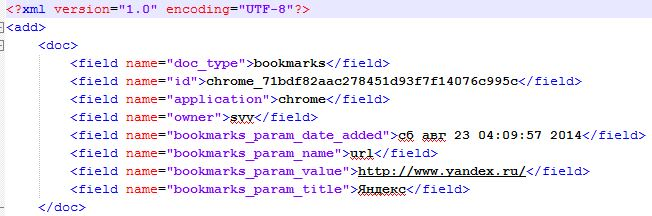
\includegraphics[width=0.7\linewidth]{ship_9}}
\caption{Файл bookmarks.XML}
\label{ship_9:ship_9}
\end{figure}

В файл history.XML (рис.~\ref{ship_10:ship_10}) добавлено поле-дата последнего посещения ресурса.

\begin{figure}[h!]
\center{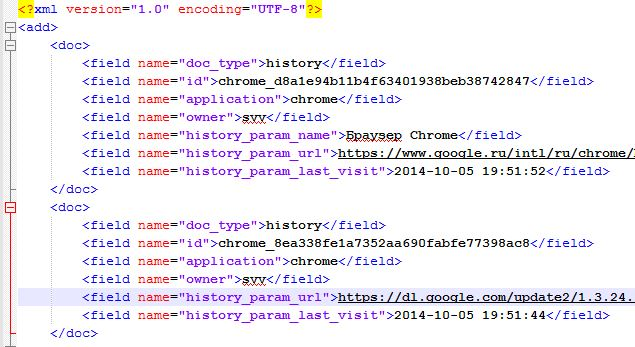
\includegraphics[width=0.8\linewidth]{ship_10}}
\caption{Файл history.XML}
\label{ship_10:ship_10}
\end{figure}

Также было реализовано преобразование данных времени начала и конца загрузки, а также о количестве занимаемого места к читаемому виду (рис.~\ref{ship_11:ship_11}).

\begin{figure}[h!]
\center{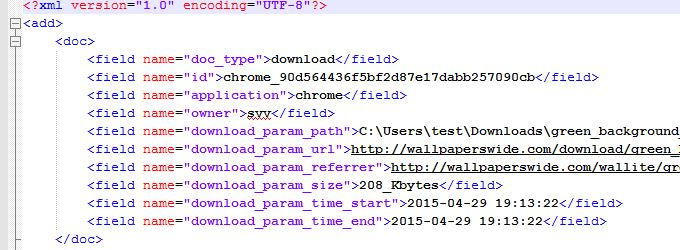
\includegraphics[width=0.8\linewidth]{ship_11}}
\caption{Файл downloads.XML}
\label{ship_11:ship_11}
\end{figure}

\clearpage
Помимо этого реализованы следующие задачи:

\begin{enumerate}
  \item присоединение модуля к общей системе coex;
  \item рекурсивный обход файловой системы для нахождения входных файлов;
  \item различие выходных данных при обработке входных от нескольких пользователей путём добавления в конец имени файла даты и количества наносекунд, прошедших с начала работы функции.
\end{enumerate}

На данный момент реализован импорт следующих данных:

\begin{enumerate}
  \item история посещений;
  \item история загруженных файлов;
  \item история поисковых запросов;
  \item список установленных расширений;
  \item информация о версии программы, подключённом аккаунте google;
  \item сохраненные данные для доступа к ресурсам(только логин).
\end{enumerate}

Список всех выходных XML-файлов приведен на рисунке~\ref{ship_12:ship_12}.

\begin{figure}[h!]
\center{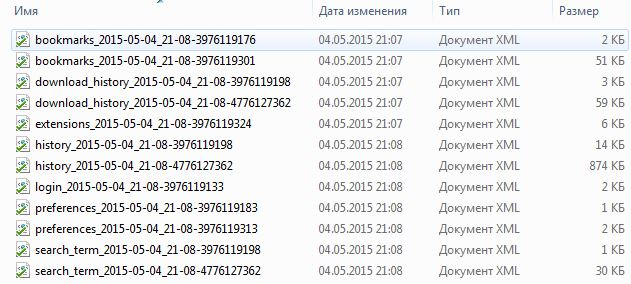
\includegraphics[width=0.7\linewidth]{ship_12}}
\caption{Файл downloads.XML}
\label{ship_12:ship_12}
\end{figure}


\newpage
\subsection{Плагин SearchProgram} % - Отчёт Макса
\subsubsection{Расположения файлов мессенджера Viber}
 
В зависимости от операционной системы (в дальнейшем ОС) у Viber разные пути установки. Для Windows XP: C:\textbackslash Documents and Settings\textbackslash \%Username\%\textbackslash Application Data\textbackslash ViberPC.
Для Windows 7, 8, 8.1, 10: C:\textbackslash Users\textbackslash \%Username\%\textbackslash AppData\textbackslash Roaming\textbackslash ViberPC (рис.~\ref{kucher_1:kucher_1}).
 
\begin{figure}[h!]
\center{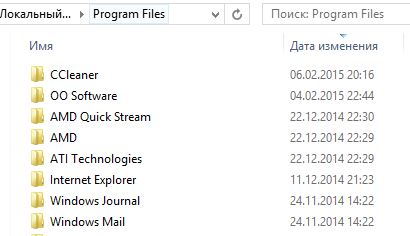
\includegraphics[width=0.8\linewidth]{kucher_1}}
\caption{ Путь к файлам Viber }
\label{kucher_1:kucher_1}
\end{figure}

\subsubsection{Описание содержимого папки «ViberPC»}

При изучении содержимого папки «ViberPC» было обнаружено, что интересующая информация содержится в папках, название которых – номер телефона (рис.~\ref{kucher_2:kucher_2}).
	

\begin{figure}[h!]
\center{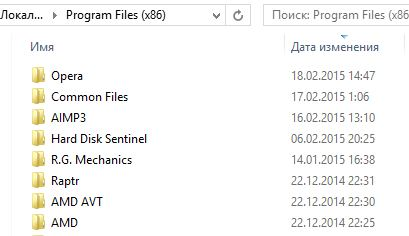
\includegraphics[width=0.8\linewidth]{kucher_2}}
\caption{ Содержимое папки с номером телефона }
\label{kucher_2:kucher_2}
\end{figure} 

\begin{itemize}
  \item Папка «Avatars» – содержит изображения пользователей;
  \item Папка «Thumbnails» – содержит все изображения, которые были отправлены и получены в ходе переписки;
	«viber.db» – база данных (далее БД), в которой хранится информация о контактах, переписках, звонках.
	БД «viber.db» – имеет формат SQLite format 3 (рис.~\ref{kucher_3:kucher_3}).
\end{itemize}
 
\begin{figure}[h!]
\center{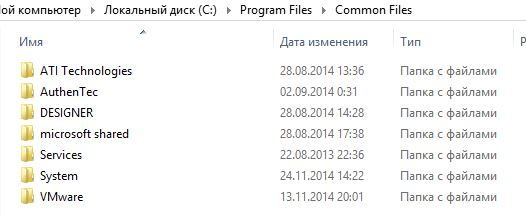
\includegraphics[width=0.3\linewidth]{kucher_3}}
\caption{ Содержимое БД «viber.db» }
\label{kucher_3:kucher_3}
\end{figure} 

\subsubsection{SQL-запросы для получения информации}

Чтобы получить все контакты и их имена был написан следующий SQL-запрос: 
\textit{Select ContactRelation.Number, Contact.FirstName from СontactRelation, Contact where Contact.ContactID = ContactRelation.ContactID}.

Чтобы получить все контакты и имена, на которые можно позвонить в Viber, нужен следующий SQL-запрос: 
\textit{Select Contact.FirstName, ContactRelation.Number from contact, PhoneNumber, ContactRelation where PhoneNumber.IsViberNumber = 1 and PhoneNumber.Number = ContactRelation.Number and ContactRelation.ContactID = Contact.ContactID}.

Чтобы связать изображение пользователя с номером телефона и именем, нужен следующий SQL-запрос:
\textit{Select Contact.FirstName, ContactRelation.Number, OriginNumberInfo.AvatarPath From OriginNumberInfo, ContactRelation, Contact Where OriginNumberInfo.Number = ContactRelation.Number and ContactRelation.ContactID = Contact.ContactID}.

Для получения информации о звонках которые осуществлялись через Viber, нужен следующий запрос: 
\textit{select Contact.FirstName, Events.Direction, datetime(Events.TimeStamp, 'unixepoch') from Contact, Events, ContactRelation where Events.EventID = (select Calls.EventID from Calls) AND Events.Number = ContactRelation.Number and ContactRelation.ContactID = Contact.ContactID}.

Для получения текста переписки с конкретным пользователем нужно знать его номер чата. Для получения всех номеров чата нужно воспользоваться следующим запросом: 
\textit{Select ChatInfo.ChatID, Contact.FirstName, ChatInfo.TokenFrom ChatInfo, ContactRelation, Contactwhere ChatInfo.Token = ContactRelation.Number and ContactRelation.ContactID = Contact.ContactID}.

Зная номер чата, можно получить текст переписки: 
\textit{select Messages.Body, Contact.FirstName, Events.Direction, Messages.ThumbnailPath, datetime(Events.TimeStamp, 'unixepoch') from messages, Events, Contact, ContactRelation where Messages.EventID = Events.EventID and Events.Number = ContactRelation.Number and ContactRelation.ContactID = Contact.ContactID and Events.ChatID = @nomer\_chata}.

\subsubsection{Описание плагина}

Плагин «TaskViber» получает точку монтирования жесткого диска, с которого, в отличии от ОС, проверяет папку «ViberPC» у всех пользователей в ОС. Если папка «ViberPC» существует, то плагин извлекает информацию из аккаунтов, под которыми авторизовались с данного компьютера. Всю найденную информацию плагин сохраняет по указанному пути программного обеспечения «COEX». В папку «Avatars» (рис.~\ref{kucher_9:kucher_9}) копируются все найденные изображения пользователей. В папку «Thumbnails» (рис.~\ref{kucher_10:kucher_10}) копируются все изображения, которые были отправлены и получены в ходе переписки. В файле «Avatar Path.txt» находятся связи между изображениями пользователей, именами и номерами телефонов. В файле «Calls.txt» находятся описание звонков, которые осуществлялись через «Viber» (с кем был звонок, во сколько и кто кому звонил). В файле «Phone book.txt» находятся все номера телефонов и имена с мобильного телефона, на котором был зарегистрирован аккаунт в «Viber». В файле «Viber book.txt» находятся все номера телефонов и имена, которым можно позвонить через «Viber». В файле «Имя/номер messages.txt» содержится переписка с пользователем «Имя/номер» (с кем велась переписка, кто кому писал, что писал и во сколько писал).

Алгоритм работы плагина «TaskViber» представлен на рисунке~\ref{kucher_4:kucher_4}, алгоритм функции WinXP --- на рисунке~\ref{kucher_5:kucher_5}. Ниже также представлены алгоритмы работы Win\_7\_8\_10 (рис.~\ref{kucher_6:kucher_6}) и Viber\_XP\_7\_8\_10 (рис.~\ref{kucher_7:kucher_7}).

Результат работы плагина представлен на рисунке~\ref{kucher_8:kucher_8}.
 

\begin{figure}[h!]
\center{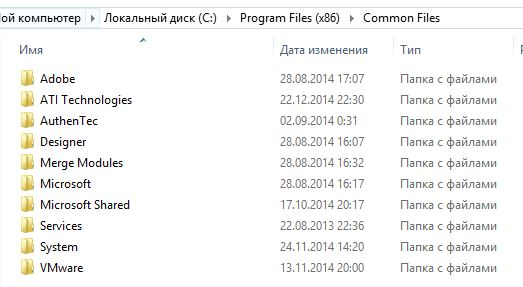
\includegraphics[width=0.6\linewidth]{kucher_4}}
\caption{ Алгоритм работы плагина }
\label{kucher_4:kucher_4}
\end{figure} 
  
\begin{figure}[h!]
\center{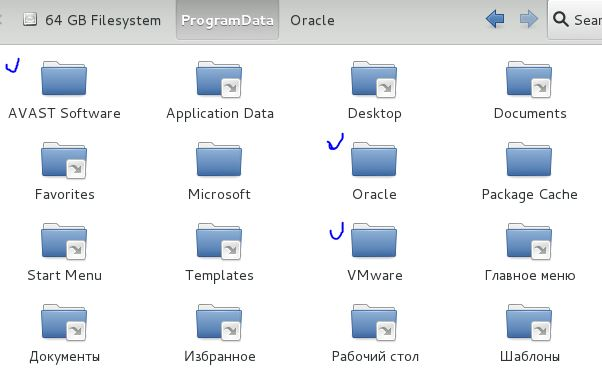
\includegraphics[width=0.6\linewidth]{kucher_5}}
\caption{ Алгоритм работы функции WinXP }
\label{kucher_5:kucher_5}
\end{figure} 

\begin{figure}[ht]
\center{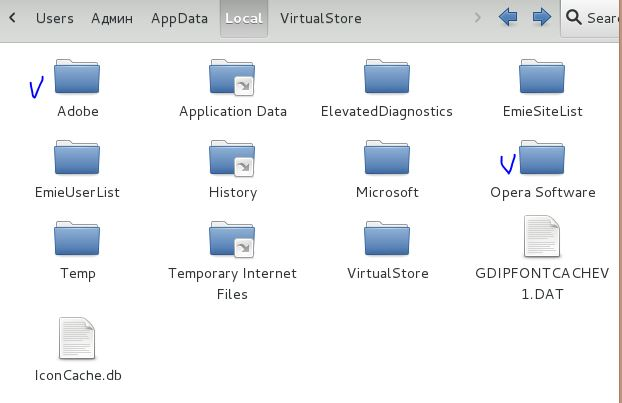
\includegraphics[width=0.6\linewidth]{kucher_6}}
\caption{ Алгоритм работы Win\_7\_8\_10 }
\label{kucher_6:kucher_6}
\end{figure} 

\begin{figure}[h!]
\center{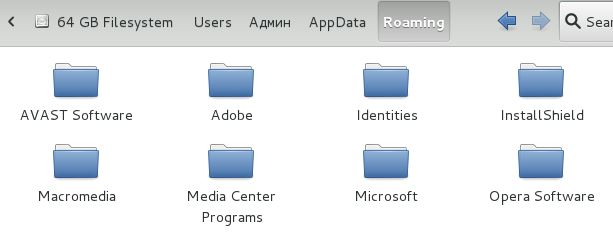
\includegraphics[width=0.5\linewidth]{kucher_7}}
\caption{ Алгоритм работы Viber\_XP\_7\_8\_10 }
\label{kucher_7:kucher_7}
\end{figure} 

\clearpage

\begin{figure}[h!]
\center{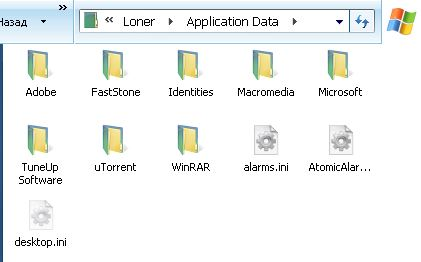
\includegraphics[width=1\linewidth]{kucher_8}}
\caption{ Результат работы плагина }
\label{kucher_8:kucher_8}
\end{figure} 

\begin{figure}[h!]
\center{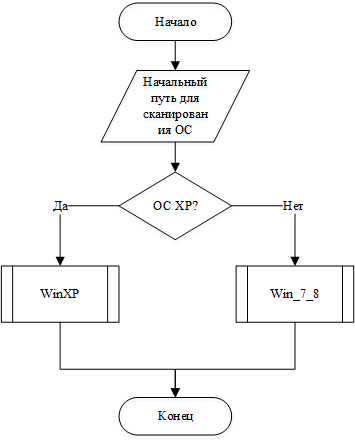
\includegraphics[width=1\linewidth]{kucher_9}}
\caption{ Содержимое папки «Avatars» }
\label{kucher_9:kucher_9}
\end{figure} 

\begin{figure}[h!]
\center{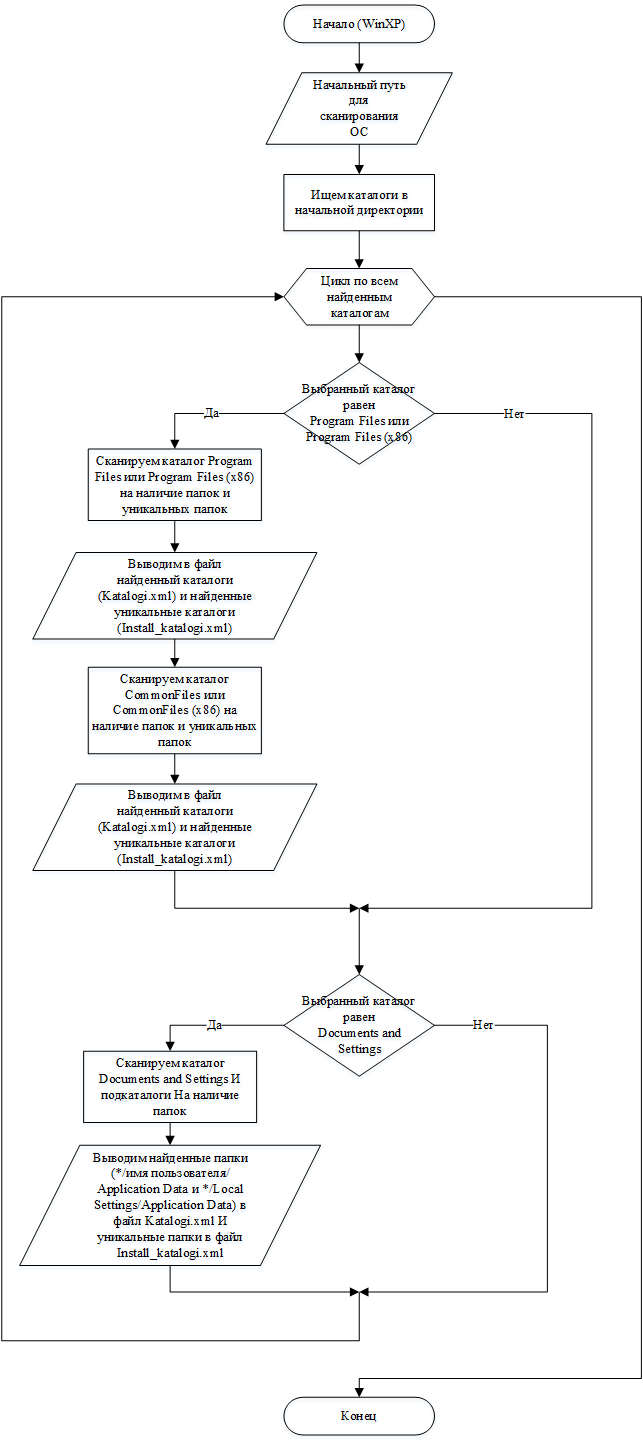
\includegraphics[width=0.8\linewidth]{kucher_10}}
\caption{ Содержимое папки «Thumbnails» }
\label{kucher_10:kucher_10}
\end{figure} 

\clearpage


\newpage
\subsection{Cбор информации из почтового клиента MS Outlook} % - Отчет Андрея
Для распространения и установки программного комплекса <<COEX>> на электронные вычислительные машины был выбран формат двоичного пакета *.deb. Данный пакет включает в себя все необходимые файлы для работы программы, а также содержит список зависимостей. Он имеет строго типизированную структуру и используется операционными системами Unix. Строго типизированная структура позволяет операционной системе узнавать все нужные элементы для установки и работы с данным пакетам вне зависимости от программного обеспечения (далее ПО), находящейся в данном Deb-пакете, узнавать зависимости программных библиотек, необходимых для запуска программного продукта, содержащегося в двоичном пакете.  Выбор данного формата пакета обусловлен возможностью его гибкой настройки для любого программного обеспечения (возможность использовать встроенные скрипты для настройки процесса установки ПО), поддержкой почти всеми операционными системами Unix. А также широкой распространенностью использования deb-пакетов в семействе операционных систем Unix в связи с высокой популярностью дистрибутивов операционных систем, в которой он распространяется.~\cite{tecmint}  

Для пакета *.deb содержащего программный комплекс <<COEX>> ранее использовалась ссылка на репозиторий содержащий данный пакет для его дальнейшей установки. При появление новой версии программного комплекса <<COEX>> создается новый deb пакет, после чего пользователю нужно было зайти на сайт программного комплекса <<COEX>>, и скачать новый deb пакет данного комплекса. Для автоматизации данного процесса было написаны две программы, а также настроена операционная утилита cron для запуска программ в определенный промежуток времени, определяемый в конфигурационном файле cron. Первая программа запрашивает у пользователя права на внесение изменений в конфигурационный файл sources.list, затем находит данный файл и вносит изменения (рисунок~\ref{ser_1:ser_1}). 

\begin{figure}[!ht]
\center{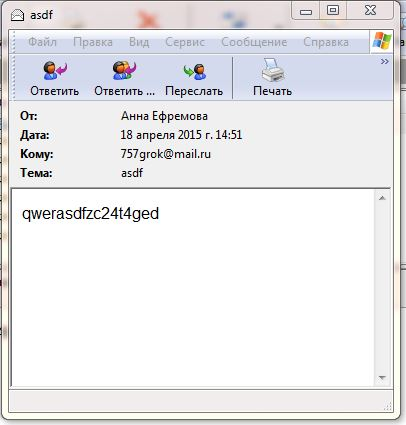
\includegraphics[width=0.7\linewidth]{ser_1}}
\caption{ Программа для внесения изменений в sources.list }
\label{ser_1:ser_1}
\end{figure}

Изменения включают в себя адрес до репозитория   в сети Internet, где хранится deb пакет программного комплекса <<COEX>>, а также запись ключа, которым подписывают скаченные файлы с репозитория, вносятся также команды по установки и обновлению пакета при скачивании через менеджера. Данные действия позволяет менеджеру обновлений операционной системы Linux следить за версиями deb пакета в репозиторие, содержащего программный комплекс <<COEX>>, при появление новой версии менеджер сообщит пользователю о возможном обновлении. Первая программа находится на сайте проекта <<COEX>>, скачивается и запускается пользователем. 

Вторая программа находится на сервере с репозиториям, и с помощью системной утилиты CRON запускается в определенное время, при наличии изменений из ветки master в системе контроля версий git (рисунок~\ref{ser_2:ser_2}).

\begin{figure}[!ht]
\center{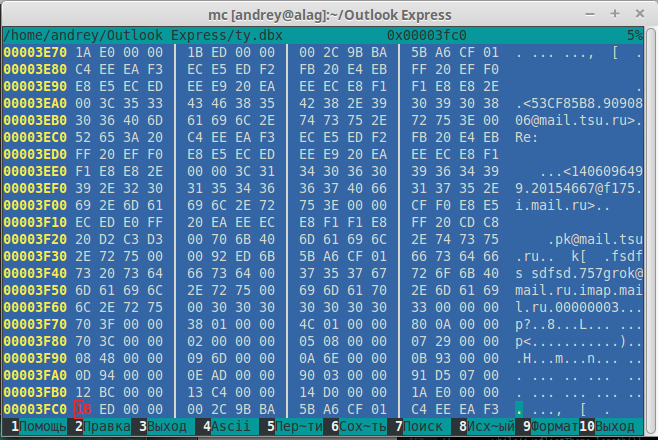
\includegraphics[width=0.7\linewidth]{ser_2}}
\caption{ Программа  для запуска сборки по времени  с помощью демона  «CRON» }
\label{ser_2:ser_2}
\end{figure}

Скрипт-программа на основе сведений из системы контроля версий GIT проекта <<COEX>>, создает версию для двоичного пакета формата deb, сам deb пакет создается при помощи скрипт-программы по созданию  deb пакета из тексты программ проекта (рисунок~\ref{ser_3:ser_3}).

\begin{figure}[!ht]
\center{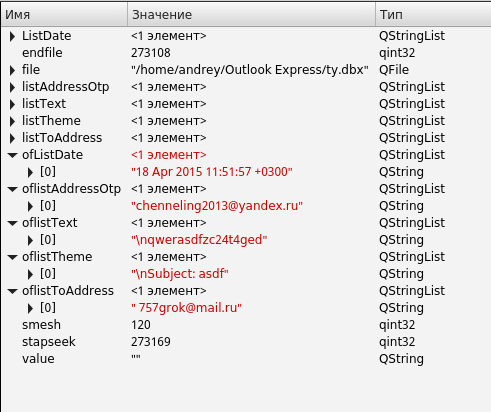
\includegraphics[width=0.7\linewidth]{ser_3}}
\caption{ Программа для присвоения версии }
\label{ser_3:ser_3}
\end{figure}

Тестирование проводилось, на операционной системе «Debian 8.4», и ее наследниках(Ubuntu(16.04), Mint (17.3))(рисунки~\ref{ser_4:ser_4}-~\ref{ser_6:ser_6}).

\begin{figure}[!ht]
\center{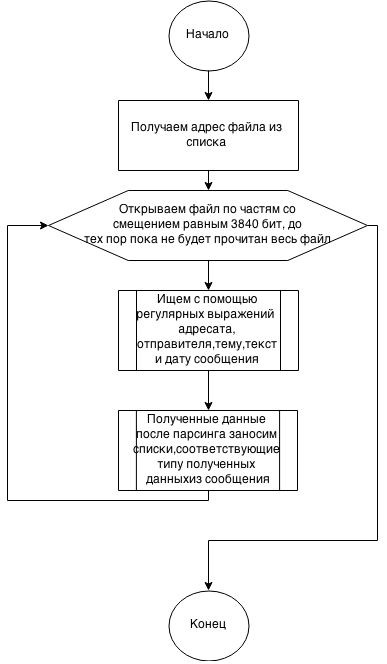
\includegraphics[width=0.7\linewidth]{ser_4}}
\caption{ Установка на Debian }
\label{ser_4:ser_4}
\end{figure}

\begin{figure}[!ht]
\center{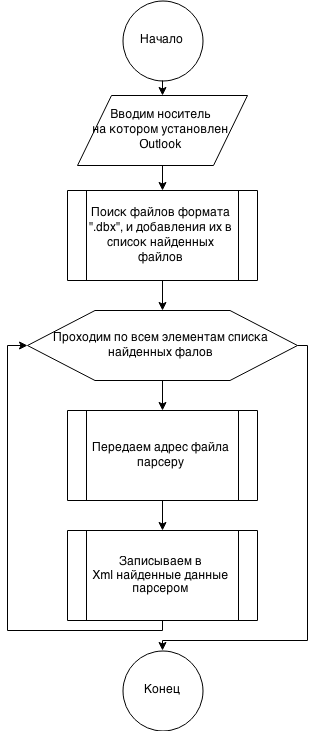
\includegraphics[width=0.7\linewidth]{ser_5}}
\caption{ Установка на Mint }
\label{ser_5:ser_5}
\end{figure}

\begin{figure}[!ht]
\center{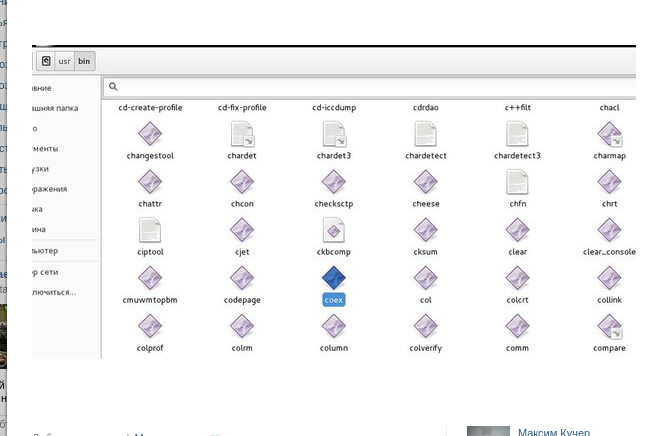
\includegraphics[width=0.7\linewidth]{ser_6}}
\caption{ Установка на Ubuntu }
\label{ser_6:ser_6}
\end{figure}

В ходе тестирования проверялось корректность работы двоичного пакета после прохождения автоматизированной сборки, также проверялась функционирование программного комплекса <<COEX>>, и корректность удаления проекта с компьютера пользователя. Результатом тестирования были выявлены проблемы с некаторами зависимостями модулей, и связи модулей c программным ядром <<COEX>>. После выявления проблем были перепроверены и исправлены зависимости, в модулях где были найдены ошибки с зависимостями. А также переделана структура пакета, для исправления проблемы взаимодействия ядра <<COEX>> и его модулей при установке через двоичный пакет.  

\clearpage


\newpage
\subsection{Cбор информации из почтового клиента Mozilla Thunderbird}  % - Отчет Юры
Целью данной работы стало исследование почтового клиента Mozilla Thunderbird, написание программного модуля для сбора сообщений и представления их в формате XML.


\subsubsection{Реализация программного модуля}

В ходе изучения приложения было выяснено расположение файлов, хранящих почтовые сообщения. Эти данные представлены в таблице~\ref{tab:data}, где:

\begin{itemize}
  \item profile\_name --- может быть любым и генерируется самой программой (например, g5bq66yo.default);
  \item server\_name --- название сервера входящей почты (например, imap.yandex.com).
\end{itemize}

\begin{table}[ht]
\caption{Местоположение и название файлов}
\label{tab:data}
\begin{center}
\begin{tabularx}{\linewidth}{|X|X|X|X|}
\hline
Протокол & Путь & Файл с входящими сообщениями & Файл с исходящими сообщениями \\
\hline
imap & C:\textbackslash Users\textbackslash User\textbackslash AppData   & INBOX & \textampersand BB4EQgQ,BEAEMAQ\\
     & \textbackslash Roaming\textbackslash Thunderbird                  &       & yBDsENQQ9BD0ES \\
     & \textbackslash Profiles\textbackslash profile\_name  &   & wQ1- \\
     & \textbackslash ImapMail\textbackslash server\_name   &   &      \\
\hline
pop3 & C:\textbackslash Users\textbackslash User\textbackslash AppData & Inbox & Sent \\
     & \textbackslash Roaming\textbackslash Thunderbird                &       &      \\
     & \textbackslash Profiles\textbackslash profile\_name             &       &      \\
     & \textbackslash Mail\textbackslash server\_name                  &       &      \\
\hline
\end{tabularx}
\end{center}
\end{table}


Для каждого почтового аккаунта, который подключен в Thunderbird, создается своя папка <<server\_name>>. Данные указаны для windows 7, 8, 8.1.


Проводник Windows не может определить расширение файлов, но при открытии любым текстовым редактором можно понять, что файлы имеют формат mbox. Mbox представляет собой текстовый файл, в котором хранятся все сообщения почтового ящика. Начало почтового сообщения определяется строкой из 5 символов: словом <<From>> с последующим пробелом.


Пример сообщения:

\begin{verbatim}
  From 
  Message-ID: <55600F73.6020804@yandex.ru>
  Date: Sat, 23 May 2015 11:26:11 +0600
  From: fgfgsr <art0rias@yandex.ru>
  User-Agent: Mozilla/5.0 (Windows NT 6.1; WOW64; rv:31.0) 
              Gecko/20100101 Thunderbird/31.7.0
  MIME-Version: 1.0
  To: yuriy94@hotmail.com
  Content-Type: text/plain; charset=utf-8; format=flowed
  Content-Transfer-Encoding: 7bit

  Little girl, little girl, Where have you been?
\end{verbatim}

В блоке с сообщением хранятся данные о дате, отправителе, получателе, версии почтового клиента, является ли письмо ответом на другое, а также заголовок и текст письма.

\subsubsection{Алгоритм работы модуля}

После открытия файл mbox разделяется на отдельные сообщения с помощью регулярного выражения <<(From \textbackslash \textbackslash r\textbackslash \textbackslash n)|(From \textbackslash \textbackslash n\textbackslash \textbackslash r)|From \textbackslash \textbackslash r|From \textbackslash \textbackslash n>>. Затем к каждому сообщению применяются регулярные выражения:

\begin{itemize}
  \item <<\textbackslash \textbackslash nDate: ([\textasciicircum \textbackslash \textbackslash n]*)\textbackslash \textbackslash n>> --- время отправки/приема сообщения;
  
  \item <<\textbackslash \textbackslash nFrom: .*([a-z][\textbackslash \textbackslash w\textbackslash \textbackslash .]*\textbackslash \textbackslash w@\textbackslash \textbackslash w[\textbackslash \textbackslash w\textbackslash \textbackslash .]*\textbackslash \textbackslash .\textbackslash \textbackslash w*).*\textbackslash \textbackslash nUser-Agent:>> --- кто отправил сообщения;
  
  \item <<\textbackslash \textbackslash nTo: .*([a-z][\textbackslash \textbackslash w\textbackslash \textbackslash .]*\textbackslash \textbackslash w@\textbackslash \textbackslash w[\textbackslash \textbackslash w\textbackslash \textbackslash .]*\textbackslash \textbackslash .\textbackslash \textbackslash w*).*\textbackslash \textbackslash nSubject:>> --- кто получил сообщение;
  
  \item <<\textbackslash \textbackslash nContent-Transfer-Encoding: 8bit\textbackslash \textbackslash s*(\textbackslash \textbackslash S.*\textbackslash \textbackslash S)\textbackslash \textbackslash s*[0-3]\textbackslash \textbackslash d\textbackslash \textbackslash .[01]\textbackslash \textbackslash d\textbackslash \textbackslash .\textbackslash \textbackslash d{4} [0-2]\textbackslash \textbackslash d:[0-5]\textbackslash \textbackslash d, [\textasciicircum \textbackslash \textbackslash n]*\textbackslash \textbackslash n>> --- текст сообщения.
\end{itemize}

Блок-схема алгоритма представлена на рисунке~\ref{teresh_1:teresh_1}.

\begin{figure}[h!]
\center{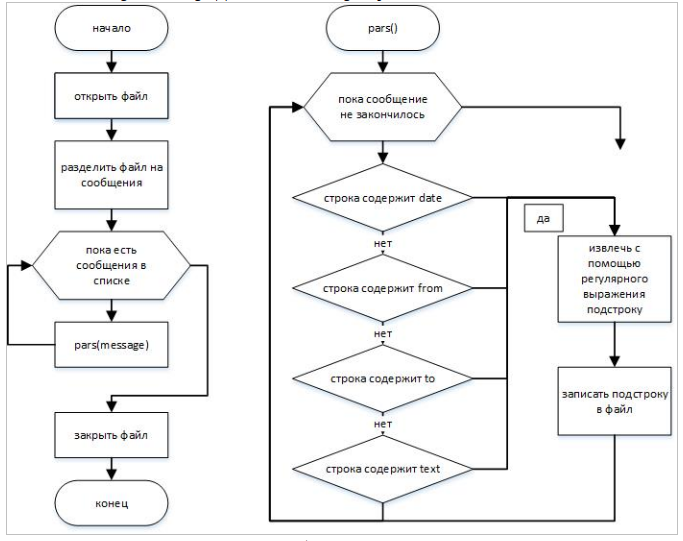
\includegraphics[width=0.9\linewidth]{teresh_1}}
\caption{Блок-схема алгоритма}
\label{teresh_1:teresh_1}
\end{figure}

\subsubsection{Структура XML-файла}

Документы XML имеют иерархическую структуру и начинаются с элемента <add> --- это начальный элемент документа (корень). Далее будут записаны n дочерних элементов <file>, где n --- количество файлов mbox. В каждый элемент <file> будут записаны m дочерних элементов <message>, где m --- количество сообщений в одном файле, в теле которых будет записано нужное нам количество полей для записи информации. В последнюю очередь записывается конечный элемент </add>.


Пример файла message\_report.xml приведен на рисунке~\ref{teresh_2:teresh_2}.


Значения полей date, from, to, text содержат время и дату, отправителя, получателя, текст сообщения соответственно. Поле name содержит полный путь к mbox файлу.

\begin{figure}[h!]
\center{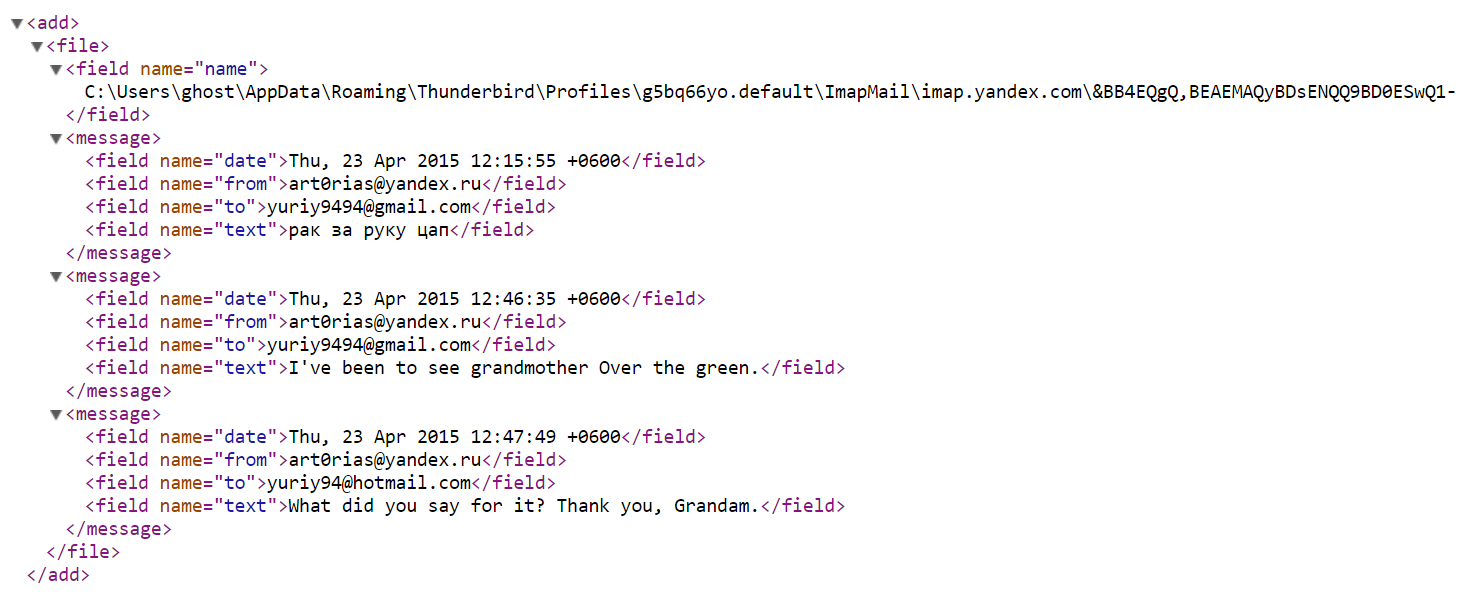
\includegraphics[width=0.9\linewidth]{teresh_2}}
\caption{Пример XML-файла}
\label{teresh_2:teresh_2}
\end{figure}
















\newpage
\subsection{Поиск медиа-файлов и извлечение мета-данных} % - Отчет Ильи
\subsection{Документирование плагинов}

На данный момент основной репозиторий находится на ресурсе GitHub. Данный ресурс использует язык разметки MarkDown (подробнее в разделе~\ref{sec:markdown}) и автоматически добавляет файл <<Readme.md>> к описанию программного модуля, если этот файл присутствует. В связи с этим было решено создать документацию плагинов, используя MarkDown. Документация должна включать в себя:

\begin{enumerate}
  \item Название плагина;
  \item Версию плагина;
  \item Автора плагина;
  \item Описание плагина;
  \item Требуемую операционную систему;
  \item Версию ПО, с которым этот плагин работает;
  \item Основные методы плагина с описанием входов и выходов.
\end{enumerate}

Результат разработанной документации можно наблюдать на странице плагина в репозитории (рис.~\ref{bok_1:bok_1}).

\begin{figure}[h!]
\center{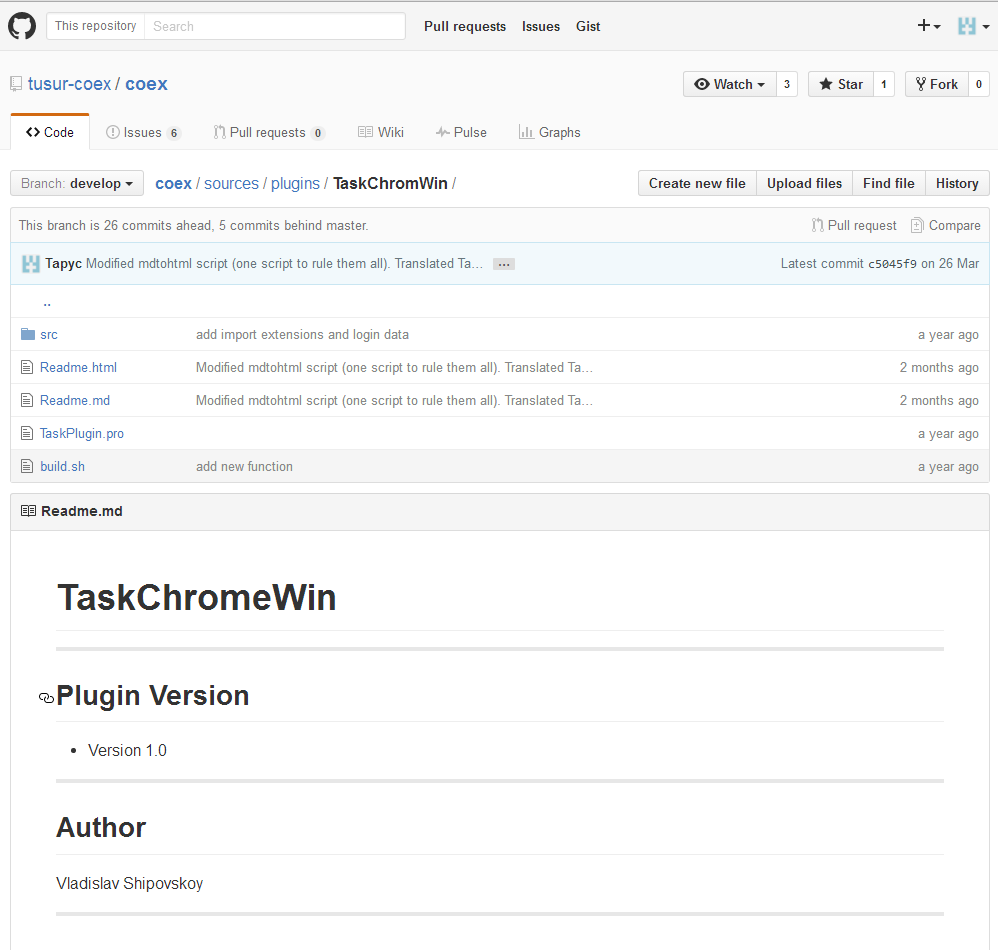
\includegraphics[width=0.8\linewidth]{bok_1}}
\caption{ Документация в веб-интерфейсе репозитория }
\label{bok_1:bok_1}
\end{figure}

Поскольку проект <<COEX>> имеет свою собственную веб-страницу, данную документацию также необходимо преобразовать в формат HTML, чтобы затем добавить на веб-страницу проекта. Для преобразования был разработан небольшой скрипт на языке Python (приложение ~\ref{apx:mdtohtml}). На рисунке ~\ref{bok_2:bok_2} можно наблюдать ту же документацию, но в формате HTML.

\begin{figure}[h!]
\center{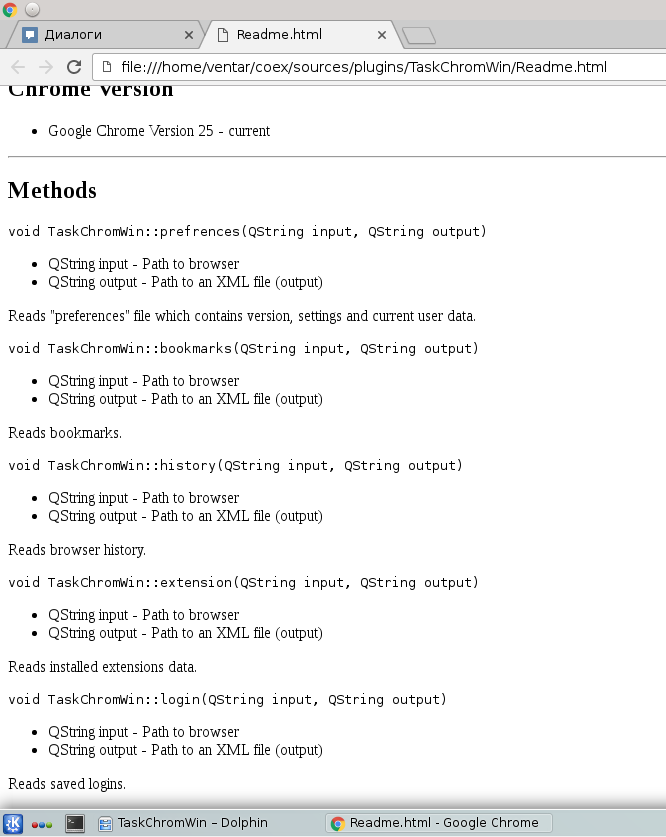
\includegraphics[width=0.9\linewidth]{bok_2}}
\caption{ Документация в формате HTML }
\label{bok_2:bok_2}
\end{figure}

\clearpage
\subsection{Разработка и внедрение копии жесткого диска}

Поскольку большое количество плагинов <<COEX>> обращается к жесткому диску для поиска тех или иных файлов, что в свою очередь создает серьезную нагрузку на него, то было решено модифицировать архитектуру проекта с целью хранения копии информации о жестком диске. Данную информацию решено было хранить как поле объекта <<config>>, к которому будут обращаться остальные плагины. Поле представляет из себя класс <<Hdd>> с атрибутом типа QList<QDir> (приложение ~\ref{apx:hddclass}). Данный тип был выбран, поскольку он позволяет хранить данные о всех директориях и файлах внутри них, а также предоставляет удобные интерфейсы для доступа к ним. Методы класса <<Hdd>>:

\begin{enumerate}
  \item Hdd::Hdd(QString path);
  \item Hdd::~Hdd();
  \item QFileInfoList getFiles(QStringList wildcardlist);
  \item QFileInfoList getFiles(QString wildcard).
\end{enumerate}

Метод <<Hdd::Hdd(QString path)>> является конструктором класса. Переменная <<path>>, подаваемая на вход метода является путем до начальной папки. Конструктор с помощью экземпляра класса <<QDirIterator>> посещает каждую папку в начальной папке и сохраняет данные о ней в переменную типа <<QDir>>, после чего добавляет эту переменную к массиву <<QList<QDir>>>, и наконец сохраняет полученный массив как поле класса. Алгоритм конструктора можно увидеть на рисунках~\ref{bok_6:bok_6} и~\ref{bok_7:bok_7}.

\begin{figure}[h!]
\center{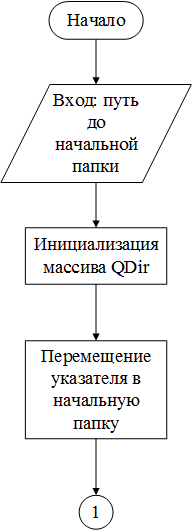
\includegraphics[width=0.3\linewidth]{bok_6}}
\caption{ Алгоритм конструктора класса <<Hdd>> }
\label{bok_6:bok_6}
\end{figure}

\begin{figure}[h!]
\center{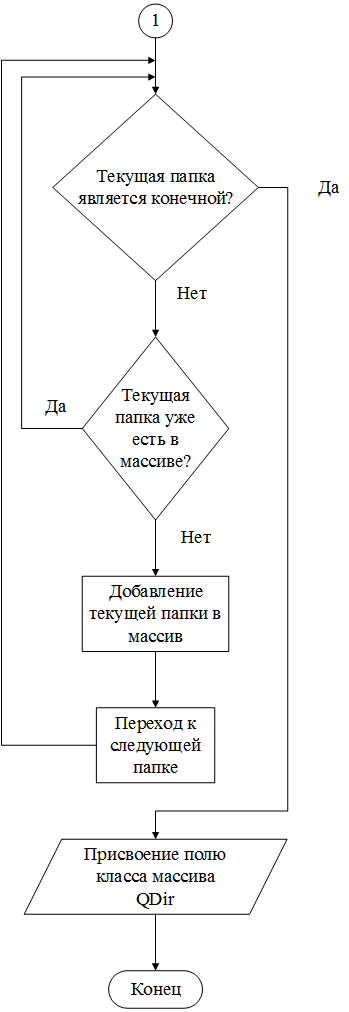
\includegraphics[width=0.5\linewidth]{bok_7}}
\caption{ Продолжение алгоритма конструктора класса <<Hdd>> }
\label{bok_7:bok_7}
\end{figure}

Метод <<Hdd::~Hdd()>> является деструктором класса.

Метод <<QFileInfoList getFiles(QStringList wildcardlist)>> возвращает объект <<QFileInfoList>> для всех файлов, которые соответствуют заданному массиву масок <<wildcardlist>>. Алгоритм метода можно увидеть на рисунке ~\ref{bok_9:bok_9}.

\begin{figure}[h!]
\center{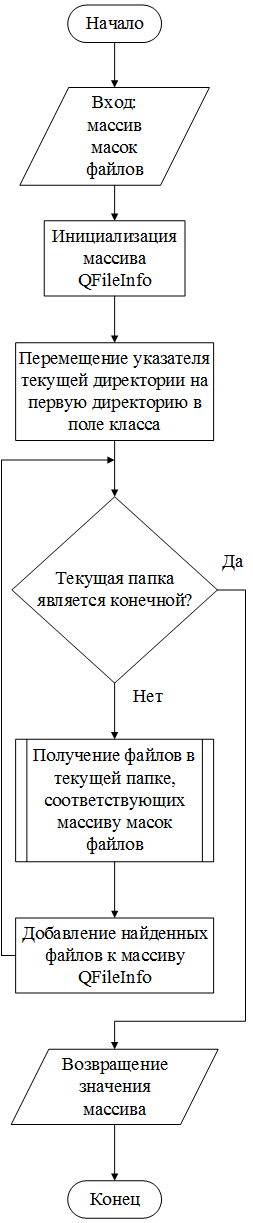
\includegraphics[width=0.3\linewidth]{bok_9}}
\caption{ Алгоритм метода <<getFiles>> класса <<Hdd>> }
\label{bok_9:bok_9}
\end{figure}

Метод <<QFileInfoList getFiles(QString wildcard)>> выполняет ту же функцию, что и прошлый метод. Он является перегрузкой прошлого метода и принимает на вход одну маску вместо массива. Алгоритм метода можно увидеть на рисунке ~\ref{bok_8:bok_8}.

\begin{figure}[h!]
\center{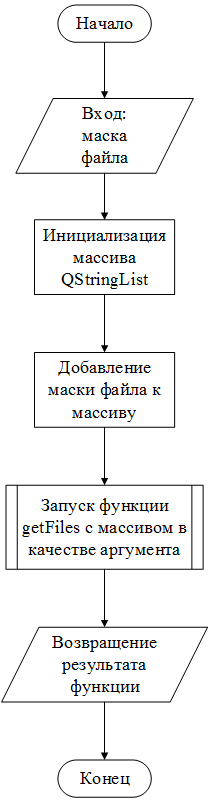
\includegraphics[width=0.3\linewidth]{bok_8}}
\caption{ Алгоритм перегруженного метода <<getFiles>> класса <<Hdd>> }
\label{bok_8:bok_8}
\end{figure}

После разработки архитектуры класса, он был внедрен в <<скелет>> проекта. Класс конструируется перед работой плагинов, но после определения операционной системы.

\begin{figure}[h!]
\center{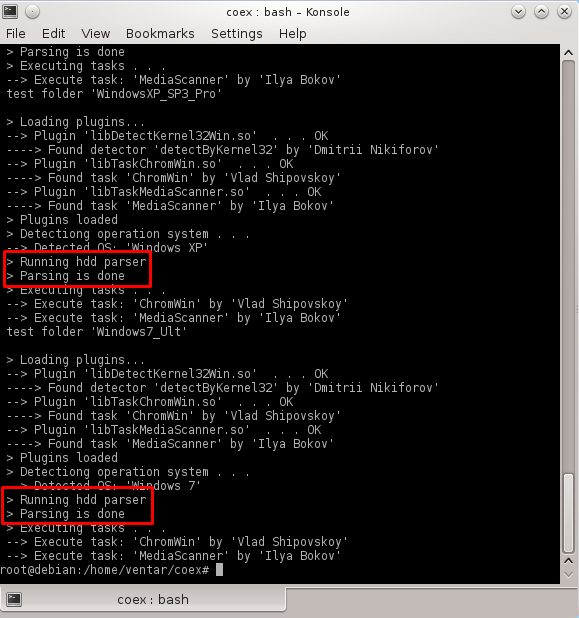
\includegraphics[width=1\linewidth]{bok_3}}
\caption{ Работа класса <<Hdd>> при запуске <<COEX>> }
\label{bok_3:bok_3}
\end{figure}

Далее необходимо было изменить плагины, таким образом, чтобы они обращались к сохраненной копии диска вместо самого диска. Таким образом были изменены два плагина - <<TaskMediaScanner>> и <<TaskChromeWin>>.

Теперь перед нами стояла задача сравнить нагрузку диска до и после внедрения класса <<Hdd>>. Поскольку нами использовался удаленный репозиторий и система контроля версий git, то это не составило проблемы по причине того, что разработка класса велась в отдельной <<ветке>>.

Было решено с помощью утилиты iotop замерить использование жесткого диска (в КБ/с) несколько раз до и после введения нового плагина и отфильтровать полученные результаты, чтобы учитывать исключительно нагрузку, создаваемую программой <<COEX>>. Для этого был разработан мультипоточный скрипт на языке Python, запускающий отдельно утилиту <<iotop>> и <<COEX>> и фильтрующий результаты, сохраняемые утилитой <<iotop>> (приложение ~\ref{apx:diskusage}):

\begin{figure}[h!]
\center{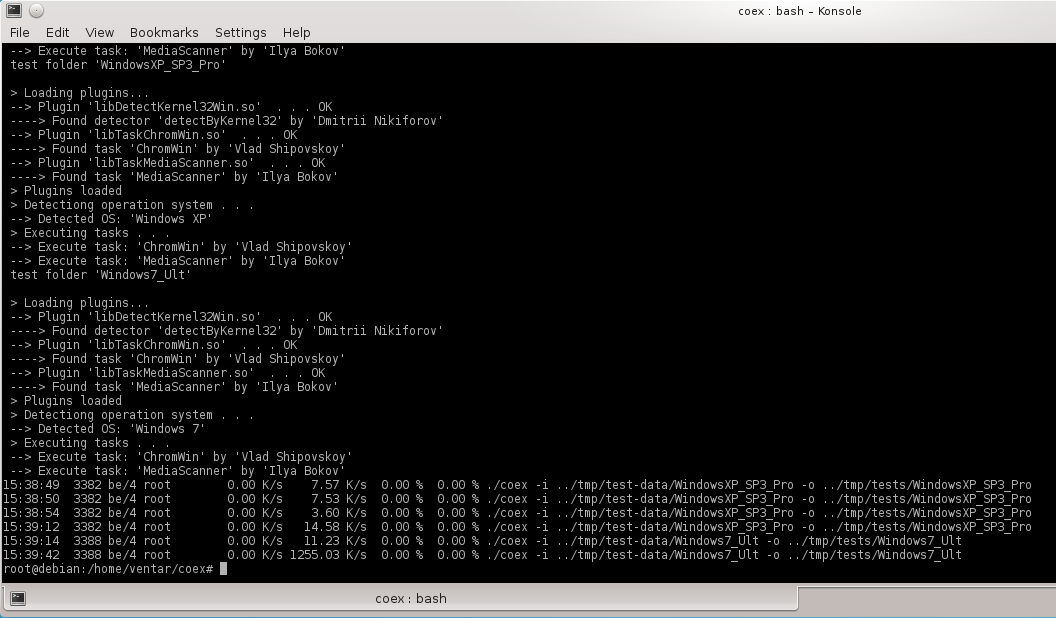
\includegraphics[width=1\linewidth]{bok_4}}
\caption{ Результат работы скрипта }
\label{bok_4:bok_4}
\end{figure}

Далее результаты были обработаны, и на основании их был построен график, показывающий нагрузку на жесткий диск до и после внедрения класса <<Hdd>>. Было решено оставить по 10 итераций на каждое измерение, поскольку после этого количества разница между итерациями была минимальна и уже прослеживалась значимая разница между измерениями.

\begin{figure}[h!]
\center{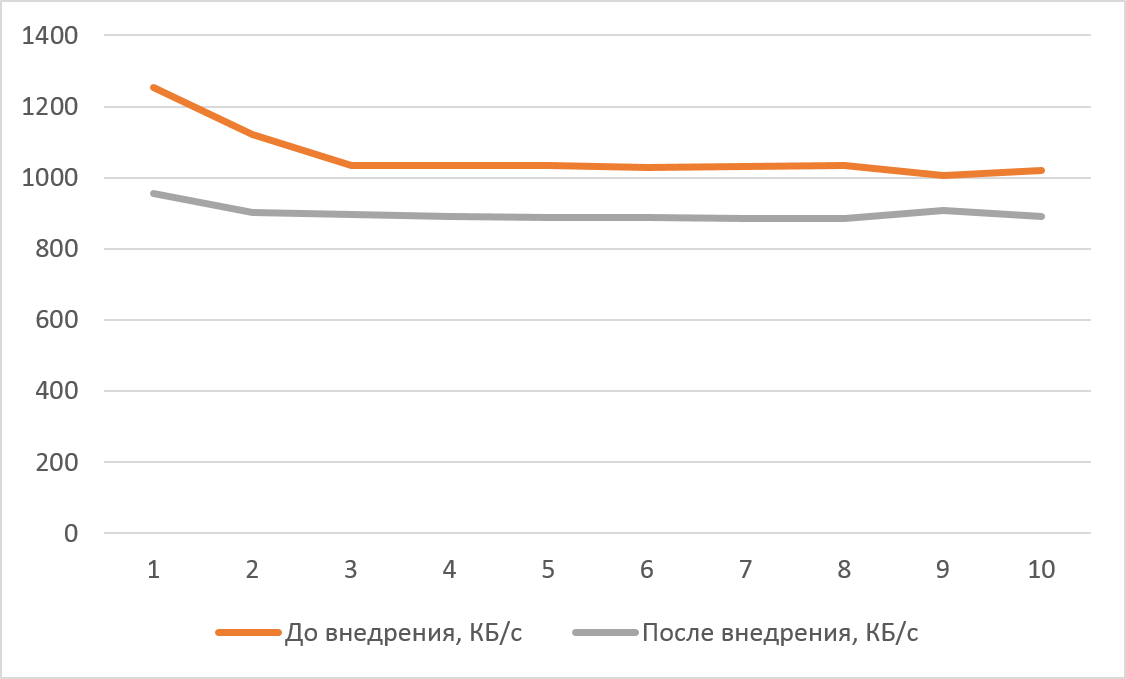
\includegraphics[width=1\linewidth]{bok_5}}
\caption{ Сравнение нагрузки на жесткий диск до и после изменения архитектуры }
\label{bok_5:bok_5}
\end{figure}

Из графика видно, что даже при изменении всего двух плагинов для использования новой архитектуры нагрузка на диск заметно снизилась. Так как на данный момент в проекте <<COEX>> имеется 17 рабочих плагинов, преобразование каждого из них должно сильно сказаться на нагрузке жесткого диска в лучшую сторону.

\clearpage


\newpage 
\subsection{Сбор и анализ информации из реестра ОС MS Windows}
Задачи текущего семестра:
\begin{itemize}
  \item Доработка плагина WinReg;
  \item Разработка веб-сайта проекта.
\end{itemize}
 
\subsection{ Доработка плагина WinReg }
 
Плагин WinReg предназначен для сбора информации из реестра Windows. Из-за особенностей формирования реестра, данный плагин был частично реализован в прошлом семестре. В этом семестре встал вопрос о его доработке. Из-за смены архитектуры и появления более срочных задач, было принято согласованное с руководством решение о временном прекращении работы над этим плагином.

\subsection{ Разработка веб-сайта проекта }

\subsubsection{ Дизайн веб-сайта проекта }

Трудно себе представить в современном мире компанию или программный продукт без персональной страницы в сети Интернет. Проекту Coex необходим свой сайт.

Современные тенденции в веб-дизайне, как и в приложениях: минимализм и простота функционала. Крупнейшие корпорации в течение последних лет выпустили гайдлайны для своих продуктов: у Microsoft – ModerUI, у Google – Flat Design.
В качестве основного направления для дизайна выбран плоский стиль с минимум сторонней графики. Используемые технологии: HTML5, CSS3, JavaScript.
Не менее важным является структура будущего макета, для этого необходимо выделить основные блоки информации, которые будут на сайте:
Информация о системе. Здесь необходимо описать, что представляет из себя система Coex и для чего она нужна;
Возможности. Что наша система может, описание плагинов;
Установка. Как установить систему, ссылки на скачивание;
Архитектура. Информация о структуре системы.
Контакты.
Исходя из всего выше, был выбран первый вариант макета: сайт-презентация (рис.~\ref{lo1:lo1}).

\begin{figure}[h!]
\center{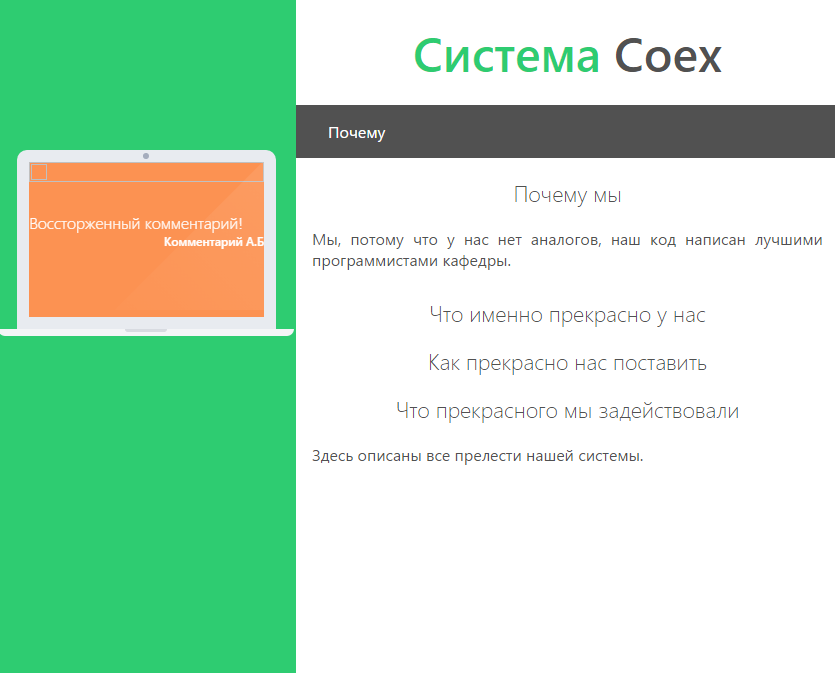
\includegraphics[width=0.8\linewidth]{lo1}}
\caption{ Первый вариант дизайна }
\label{lo1:lo1}
\end{figure}

Позднее данный дизайн отклонён из-за нерационального использования пространства веб-страницы и сложности расположение контента в пользу нового варианта (рис.~\ref{lo2:lo2}).

\begin{figure}[h!]
\center{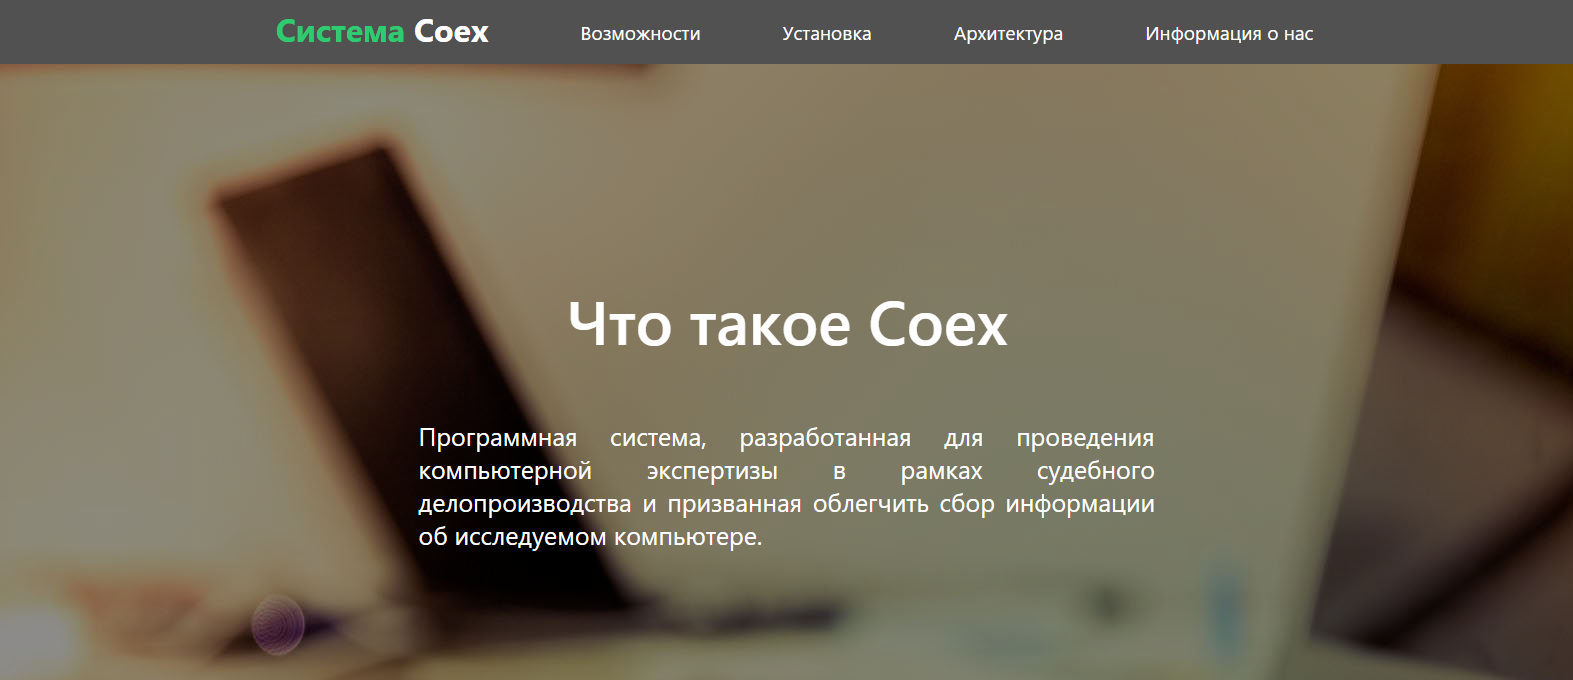
\includegraphics[width=0.8\linewidth]{lo2}}
\caption{ Новый вариант дизайна }
\label{lo2:lo2}
\end{figure}

Был выбран вариант с одним блоком информации на одну страницу прокрутки – так можно акцентировать внимание посетителя на необходимых деталях, не отвлекая его по мелочам.

\subsubsection{ Вёрстка дизайна } 

Как было сказано ранее, используются технологии HTML5 и CSS3, что позволяет существенно сократить код стилей и нагляднее писать код страницы. Минусом данного подхода является требование к наличию у посетителей последних версию интернет браузеров, но, как показывает статистика, количество таких пользователей превалирует (рис.~\ref{lo3:lo3}).

\begin{figure}[h!]
\center{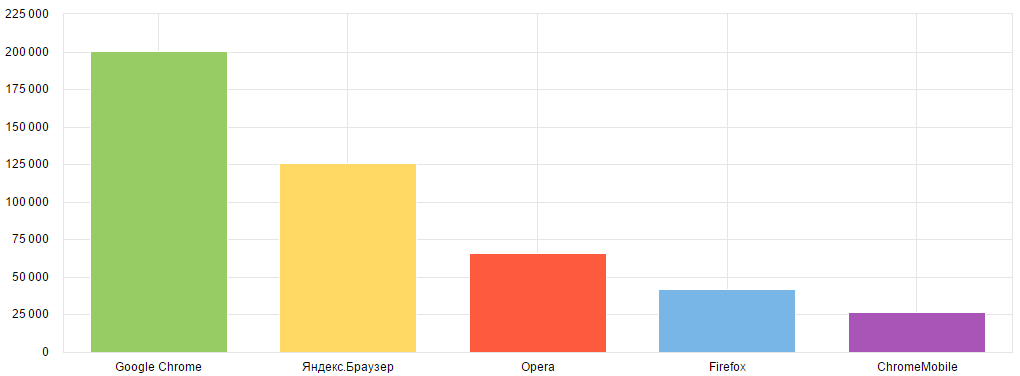
\includegraphics[width=0.8\linewidth]{lo3}}
\caption{ Количество посетителей с различными браузерами }
\label{lo3:lo3}
\end{figure}

Для обеспечения поддержки мобильных устройств и устройств с нестандартным разрешение экрана в вёрстке максимально использованы новые возможности CSS3, такие как flex-box, box-sizing и другие (рис.~\ref{lo4:lo4}).

\begin{figure}[h!]
\center{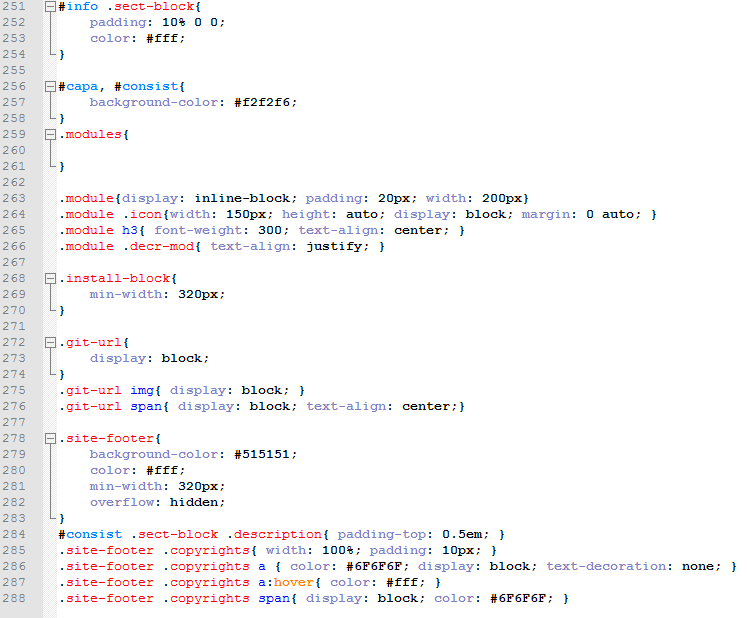
\includegraphics[width=0.8\linewidth]{lo4}}
\caption{ Часть кода CSS-стилей }
\label{lo4:lo4}
\end{figure}

\subsubsection{ Регистрация домена }

Был подобран и зарегистрирован домен coex.su, параллельно с этим изучены принципы построения DNS серверов и NX записи (рис.~\ref{lo5:lo5}).

\begin{figure}[h!]
\center{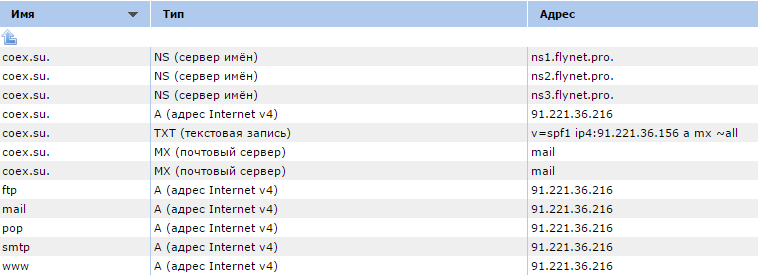
\includegraphics[width=0.8\linewidth]{lo5}}
\caption{ Пример NX-записей для домена coex.su }
\label{lo5:lo5}
\end{figure}

\subsubsection{ Настройка WEB-сервера }

Для сайта был запущен и настроен веб-сервер apache в связке с nginx. В дальнейшем апач будет <<отдавать>> посетителям динамический контент, такой как новости, а nginx – статический: исходные коды программы с репозитария, картинки, видео и прочее (рис.~\ref{lo6:lo6}).

\begin{figure}[h!]
\center{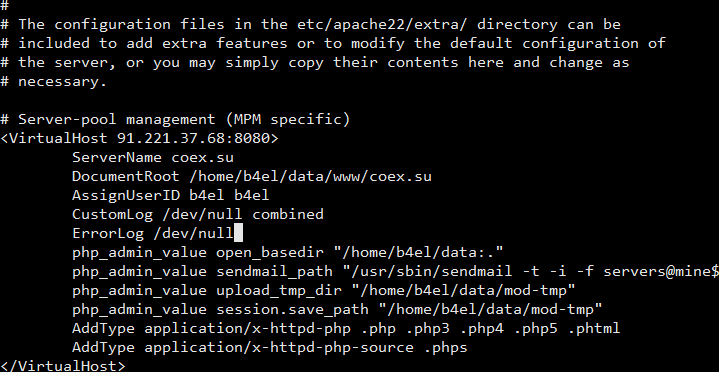
\includegraphics[width=0.8\linewidth]{lo6}}
\caption{ Часть конфига Apache }
\label{lo6:lo6}
\end{figure}

\subsubsection{ Контент }

Для наполнения сайта были написаны тексты, описывающие систему, ее части и возможности. Для каждого плагина была подготовлена своя иконка (рис.~\ref{lo7:lo7}) и описание.

\begin{figure}[h!]
\center{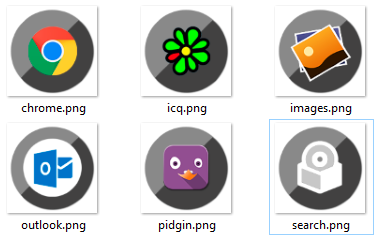
\includegraphics[width=0.8\linewidth]{lo7}}
\caption{ Иконки для плагинов }
\label{lo7:lo7}
\end{figure}

\subsubsection{ Планы на будущий семестр }

В планах на будущее стоит завершение дизайна сайта и перенос его на CMS, наполнение контентом, проведение SEO разметки.

\clearpage











\newpage
\section*{Заключение}
\addcontentsline{toc}{section}{Заключение}
В данном семестре нашей группой была выполнена часть работы по созданию автоматизированного программного комплекса для проведения компьютерной экспертизы, проанализированы дальнейшие перспективы и поставлены цели для дальнейшего развития проекта.
 
 
 \newpage
 \renewcommand{\refname}{Список использованных источников}
 \bibliography{lit}

 \ESKDappendix{Обязательное}{\normalfont Компакт-диск}
 Компакт-диск содержит: 
 \begin{itemize}
 \item электронную версию пояснительной записки в форматах *.tex и *.pdf;
 \item актуальную версию программного комплекса для проведения компьютерной экспертизы;
 \item тестовые данные для работы с программным комплексом;
 \item документацию к проекту в html-формате.
 \end{itemize}
 
\end{document}
